\documentclass{sigchi}

% Use this command to override the default ACM copyright statement
% (e.g. for preprints).  Consult the conference website for the
% camera-ready copyright statement.


%% EXAMPLE BEGIN -- HOW TO OVERRIDE THE DEFAULT COPYRIGHT STRIP -- (July 22, 2013 - Paul Baumann)
% \toappear{Permission to make digital or hard copies of all or part of this work for personal or classroom use is      granted without fee provided that copies are not made or distributed for profit or commercial advantage and that copies bear this notice and the full citation on the first page. Copyrights for components of this work owned by others than ACM must be honored. Abstracting with credit is permitted. To copy otherwise, or republish, to post on servers or to redistribute to lists, requires prior specific permission and/or a fee. Request permissions from permissions@acm.org. \\
% {\emph{CHI'14}}, April 26--May 1, 2014, Toronto, Canada. \\
% Copyright \copyright~2014 ACM ISBN/14/04...\$15.00. \\
% DOI string from ACM form confirmation}
%% EXAMPLE END -- HOW TO OVERRIDE THE DEFAULT COPYRIGHT STRIP -- (July 22, 2013 - Paul Baumann)


% Arabic page numbers for submission.  Remove this line to eliminate
% page numbers for the camera ready copy 

%\pagenumbering{arabic}

% Load basic packages
\usepackage{balance}  % to better equalize the last page
\usepackage{graphics} % for EPS, load graphicx instead 
%\usepackage[T1]{fontenc}
\usepackage{txfonts}
\usepackage{times}    % comment if you want LaTeX's default font
\usepackage[pdftex]{hyperref}
% \usepackage{url}      % llt: nicely formatted URLs
\usepackage{color}
\usepackage{textcomp}
\usepackage{booktabs}
\usepackage{ccicons}
\usepackage{todonotes}
\usepackage{subfigure}
\usepackage{multirow}

% llt: Define a global style for URLs, rather that the default one
\makeatletter
\def\url@leostyle{%
  \@ifundefined{selectfont}{\def\UrlFont{\sf}}{\def\UrlFont{\small\bf\ttfamily}}}
\makeatother
\urlstyle{leo}

% To make various LaTeX processors do the right thing with page size.
\def\pprw{8.5in}
\def\pprh{11in}
\special{papersize=\pprw,\pprh}
\setlength{\paperwidth}{\pprw}
\setlength{\paperheight}{\pprh}
\setlength{\pdfpagewidth}{\pprw}
\setlength{\pdfpageheight}{\pprh}

% Make sure hyperref comes last of your loaded packages, to give it a
% fighting chance of not being over-written, since its job is to
% redefine many LaTeX commands.
\definecolor{linkColor}{RGB}{6,125,233}
\hypersetup{%
  pdftitle={SIGCHI Conference Proceedings Format},
  pdfauthor={LaTeX},
  pdfkeywords={SIGCHI, proceedings, archival format},
  bookmarksnumbered,
  pdfstartview={FitH},
  colorlinks,
  citecolor=black,
  filecolor=black,
  linkcolor=black,
  urlcolor=linkColor,
  breaklinks=true,
}

% create a shortcut to typeset table headings
% \newcommand\tabhead[1]{\small\textbf{#1}}

% End of preamble. Here it comes the document.
\begin{document}
\author{
  Yvonne Chen\\
  \texttt{evechen@uw.edu}
  \and
  Eleanor O'Rourke\\
  \texttt{eorourke@cs.washington.edu}
}
\title{Visualizing Student Problem-Solving Data}


\maketitle

\begin{abstract}
Abstract goes here
\end{abstract}


%\keywords{Technology in the classroom; tablets for education; adaptive learning environments.}

%\category{H.5.0.}{Information Interfaces and Presentation}{General}

\section{Introduction}
Intro here

\section{Related Work}
A large body of research has explored methods of integrating technology into in-person classrooms and using technology to deliver education online. We review this research focusing on technology-delivered curriculums, systems that expose student data for teachers, and adaptive learning environments.

\subsection{Exposing Student Data for Teachers}
Education research shows that teacher behavior has a strong impact on student achievement \cite{Hill2005, Wentzel2002, Reeve2004, Wright1997}, and that teachers can benefit from the availability of real-time student data \cite{Balaam2010, Koile2006, Lazar2007}. For example, Koile found that when an instructor was given access to student problem solutions through tablet-based technology in real-time, the instructor devoted 75\% of class time responding to student misunderstandings \cite{Koile2006}. With access to real-time data, research suggests that instructors can intervene during a lesson when students are confused \cite{Hickey2014}, alter the pace or content of instruction based on student engagement \cite{Balaam2010}, immediately identify and assist students who are struggling \cite{Lazar2007}, and choose topics of focus based on aggregates of student responses \cite{Koile2006}. 

A number of technologies have been developed for exposing student data for teachers. One technology that is often used in lecture-based classes is the ``student response system'' or ``clicker,'' which is used to poll students on multiple-choice questions during class \cite{Dangel08, Lazar2007}. A similar application designed for small classes is Plickers \cite{Plickers}. With the Plickers smartphone app, the teacher can scan the classroom while students hold up QR codes identifying a multiple-choice answer \cite{Plickers}. Researchers have also explored methods of providing instructors with access to student data outside of instruction time to monitor longer term academic progress \cite{Zhang2015, Arnold2012}. Kim et.\ al.\ developed a system for compiling student responses to MOOC exercise problems, which teachers reported were useful for capturing student thought processes, identifying misconceptions, and engaging students with content \cite{Kim2015}.

In this work, we explore methods of exposing rich problem-solving data to elementary school teachers in real-time. Through a longitudinal study, we explore how teacher behavior is impacted by exposing information about student misconnects and progress through curriculum material.

Whether viewed in real time or after the fact, teachers benefit from the availability of student data. Accessed in real time, student data affords immediate intervention. In a study by Koile, students used Tablet PCs to complete exercise problems during class time. The instructor could access their answers right away on her own device. Based on the students? answers, the instructor devoted 75\% of course time responding to misunderstandings of course material, and would delay or hasten presentation of new material as appropriate \cite{Koile2006}. With real time student data, instructors can intervene during a lesson when students are confused \cite{Hickey2014}, alter the pace or content of instruction based on student engagement \cite{Balaam2010}, immediately identify and assist students who are struggling \cite{Lazar2007}, and choose topics of focus based on aggregates of student responses \cite{Koile2006}.

When timely intervention is less critical, instructors can view data outside of instruction time to
monitor longer term academic progress \cite{Zhang2015, Arnold2012}. Kim et al developed an online system for teachers to author video lectures containing integrated multimedia exercises. The system compiled student responses as they completed exercises, and teachers reported that they were useful for ?capturing students? thought processes, identifying misconceptions, and engaging students with content? \cite{Kim2015}. Even basic classroom response systems, which poll students to choose one out of a set of pre-defined responses, give teachers a quick aggregate overview of student understanding \cite{Lazar2007}.

While research shows that student data can help teachers understand misconceptions and how they spend class time, very little is known about how to visualize student data to most effectively communicate with teachers. We have not encountered any papers that study the design of visualizations of student data. Enlearn has implemented two different methods of visualizing student data in real-time for teachers, however, both of their designs have had usability and readability problems when tested in classrooms. This shows how challenging it is to create effective visualizations for communicating student data in real-time. Enlearn?s first design, shown in Figure 1a, displays a table view of student problem solving pace and correctness. While this visualization provides information about the progress of individual students, it communicates nothing about the specific concepts that students are struggling with. Enlearn?s second design, shown in Figure 1b, displays a graph view of student problem solving that is organized by concept. While this displays information about the concepts that students are struggling with, there is no way for teachers to see which individuals are struggling. Most importantly, neither visualization provides teachers with actionable suggestions about how to assist students who are struggling. Prior work shows the utility of communicating student data for instructors, and Enlearn?s experiences with their current visualizations shows the challenge of designing effective means of communicating data, especially in real time for busy teachers. This motivates our desire to improve and strengthen the data visualization for the Enlearn software.

\begin{figure*}[t]
\centering
\subfigure[]{\label{fig:TeacherLesson}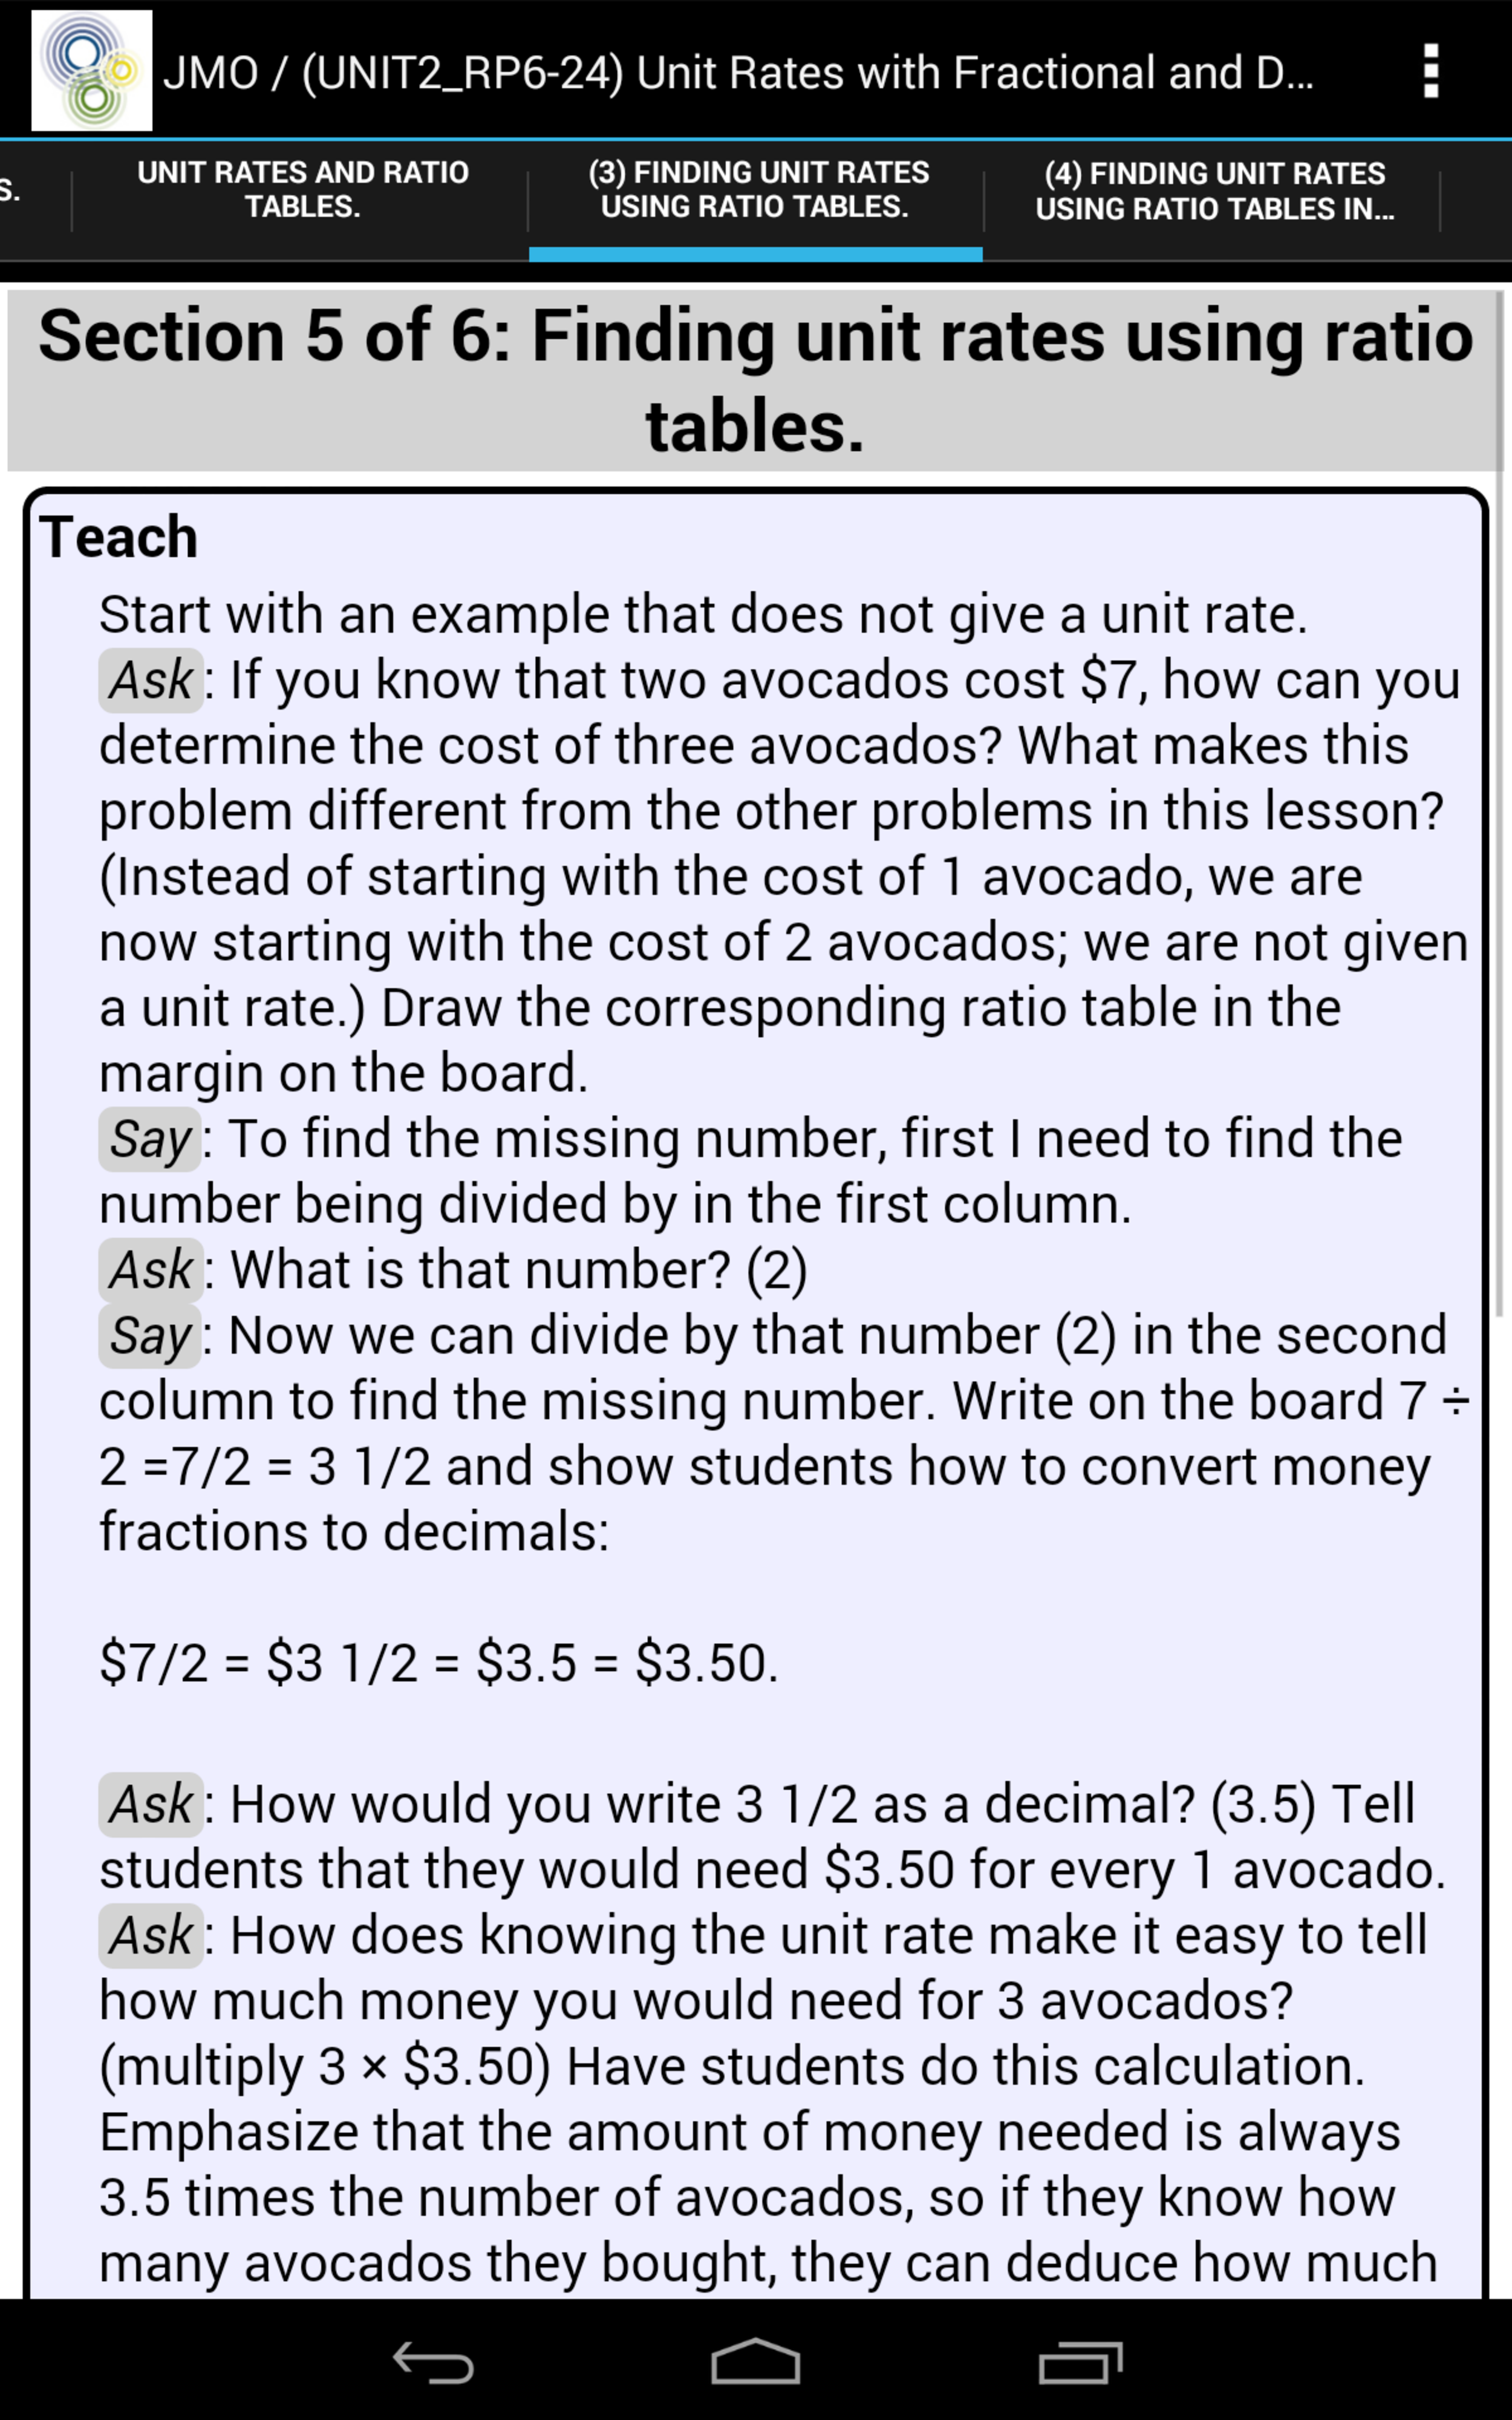
\includegraphics[width=40mm]{images/TeacherLesson.pdf}} \hspace{1em}%
\subfigure[]{\label{fig:TeacherStartProbems}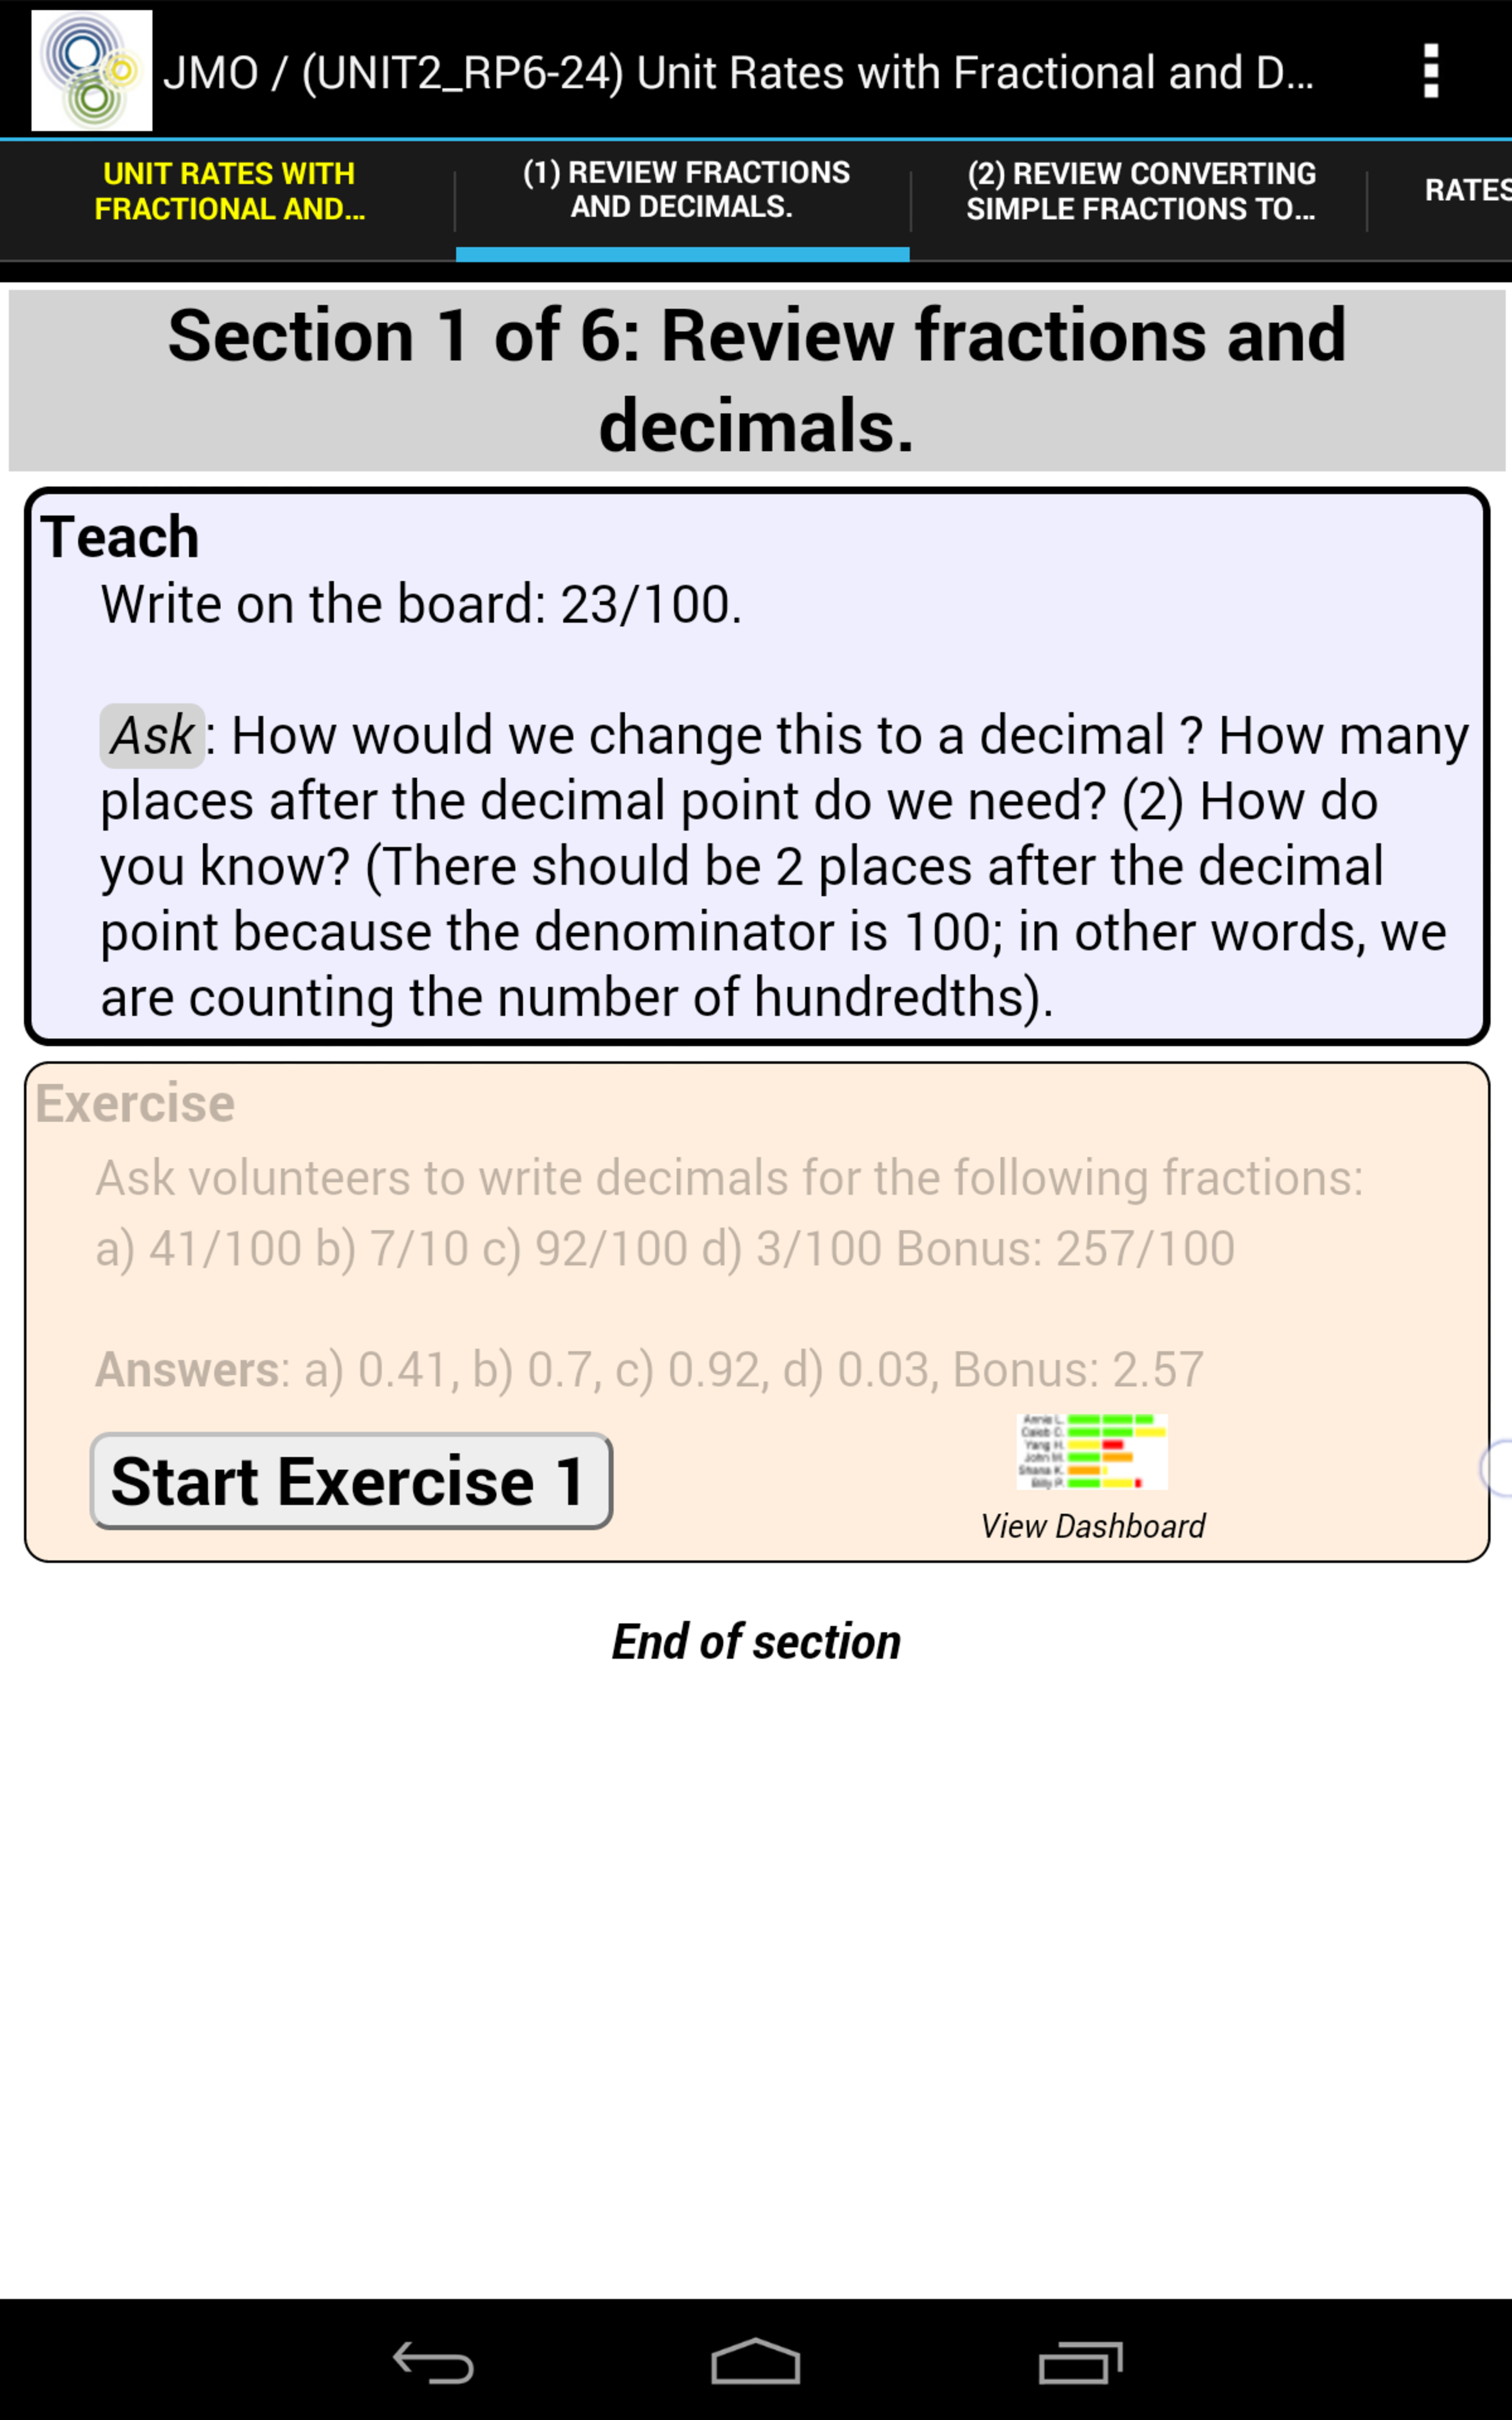
\includegraphics[width=40mm]{images/TeacherEX.pdf}} \hspace{1em}%
\subfigure[]{\label{fig:TeacherDashboard}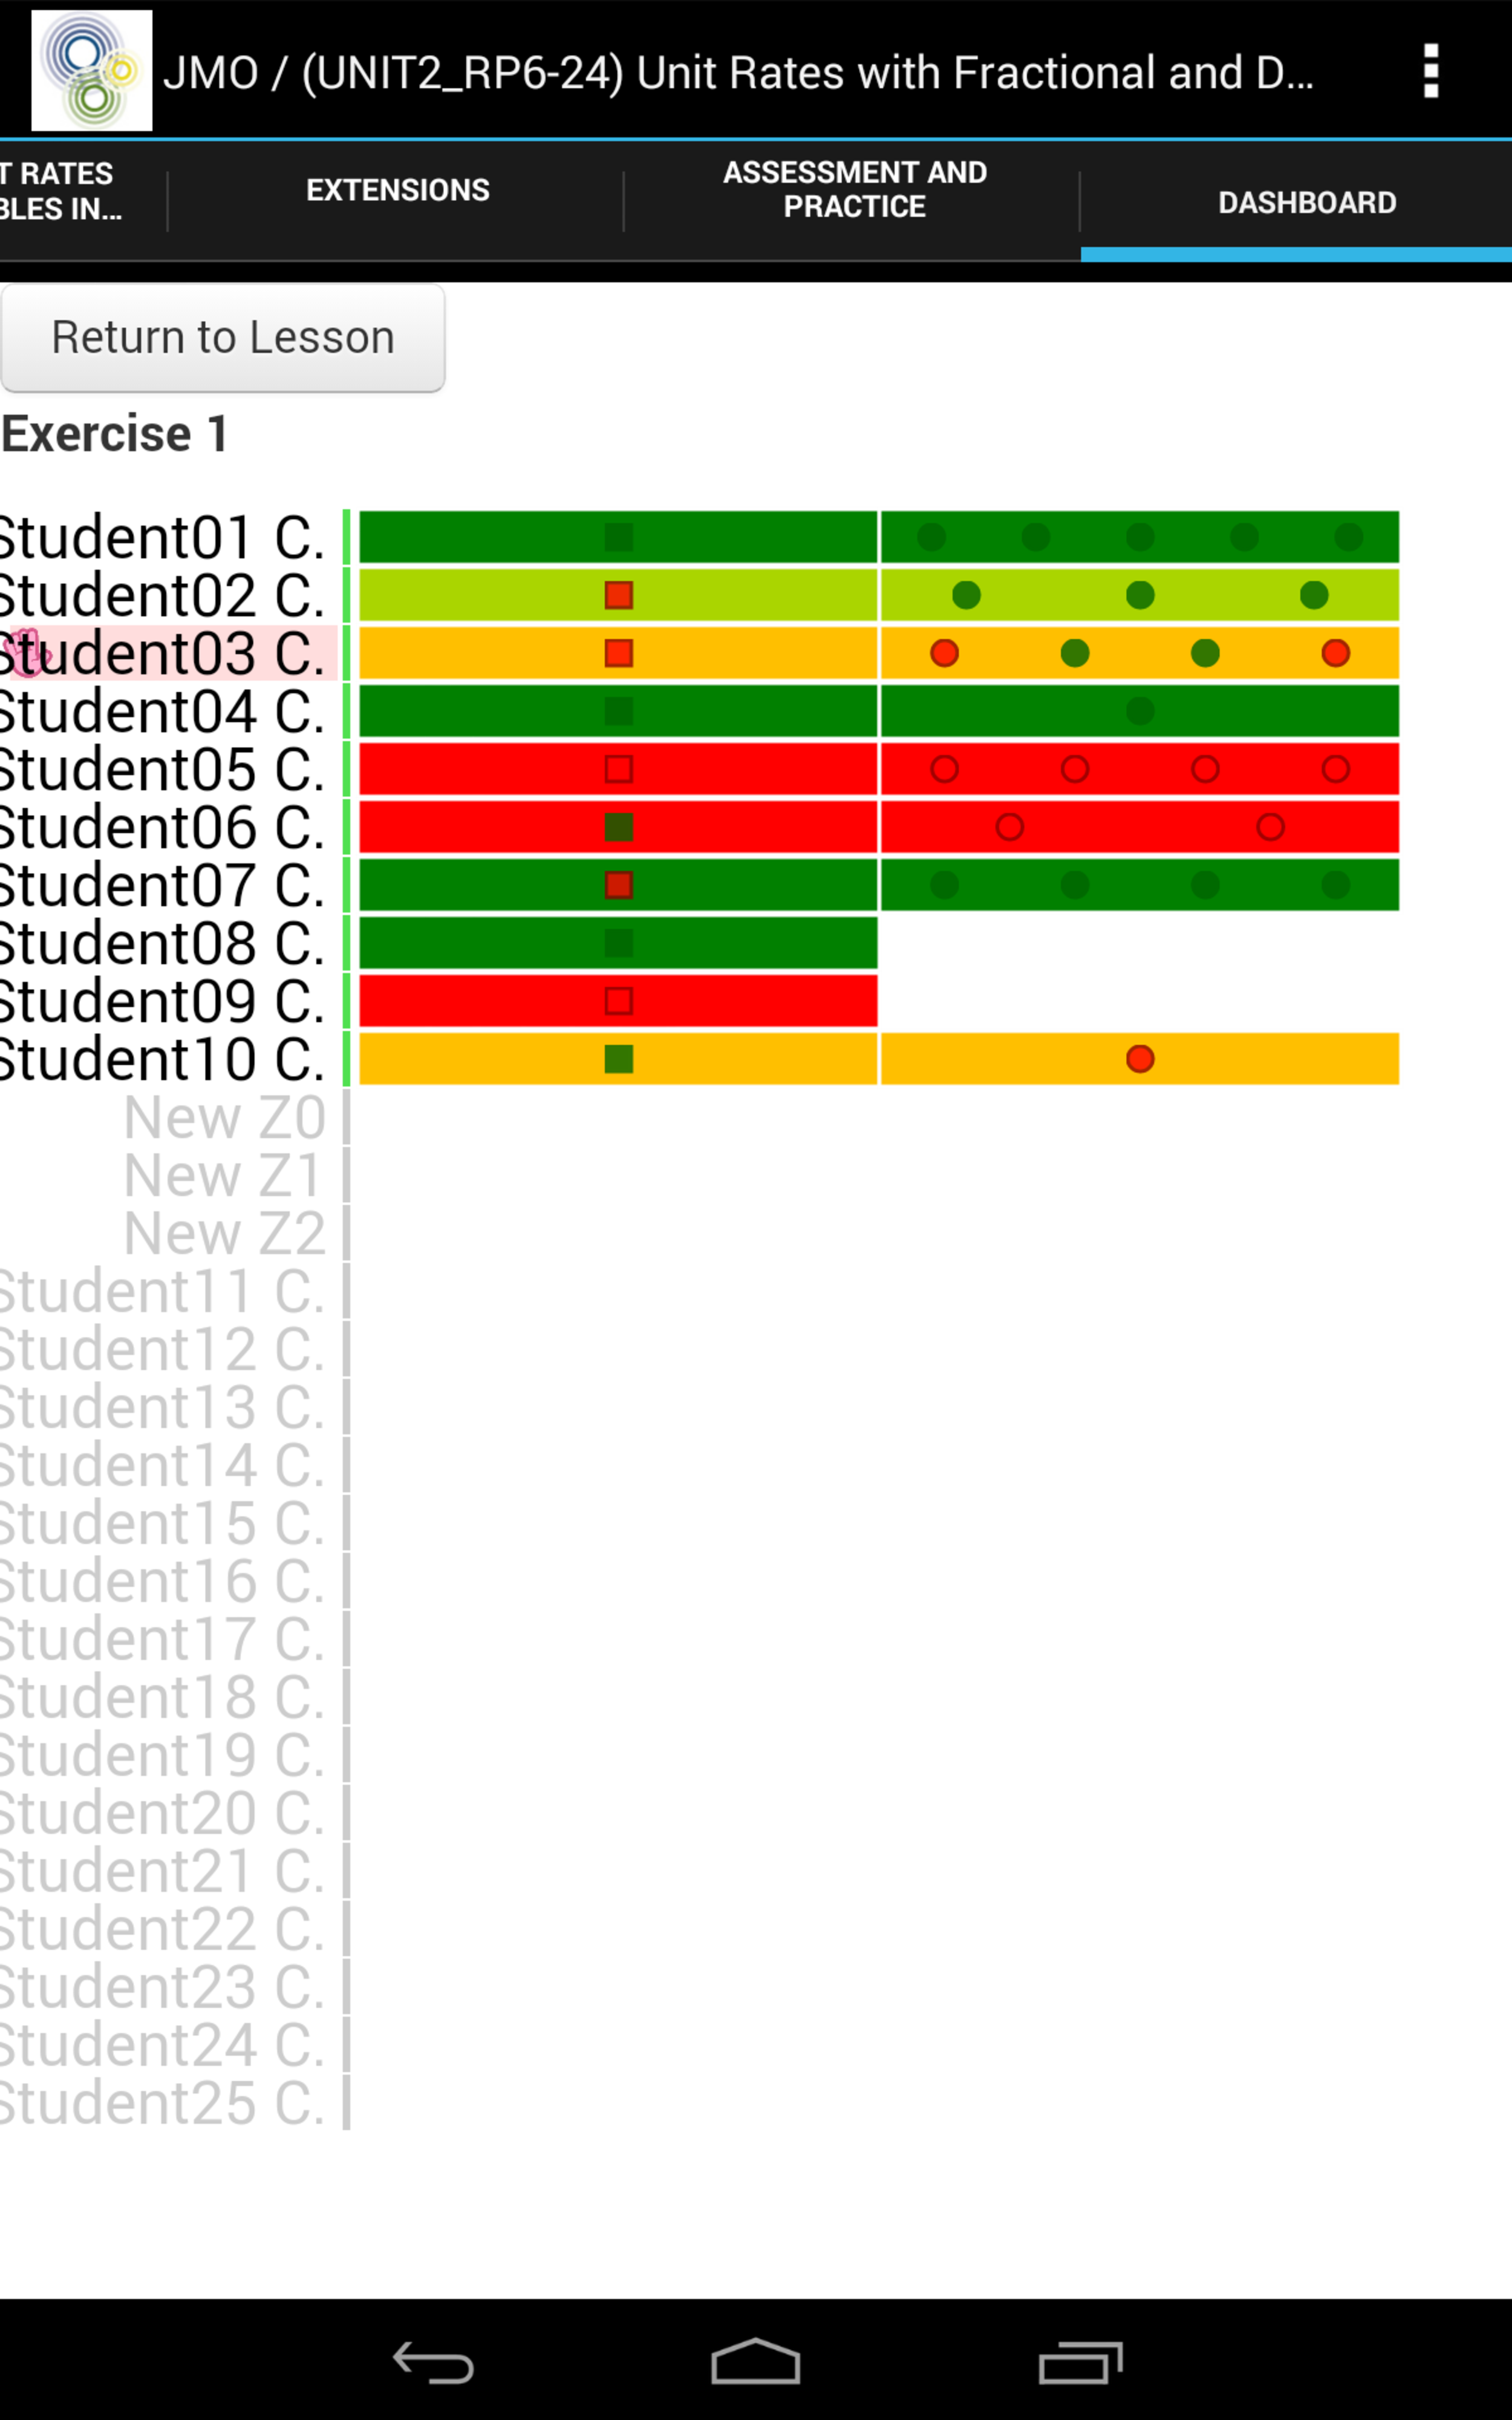
\includegraphics[width=40mm]{images/TeacherDashboard.pdf}} \hspace{1em}%
\subfigure[]{\label{fig:StudentProblemSolving}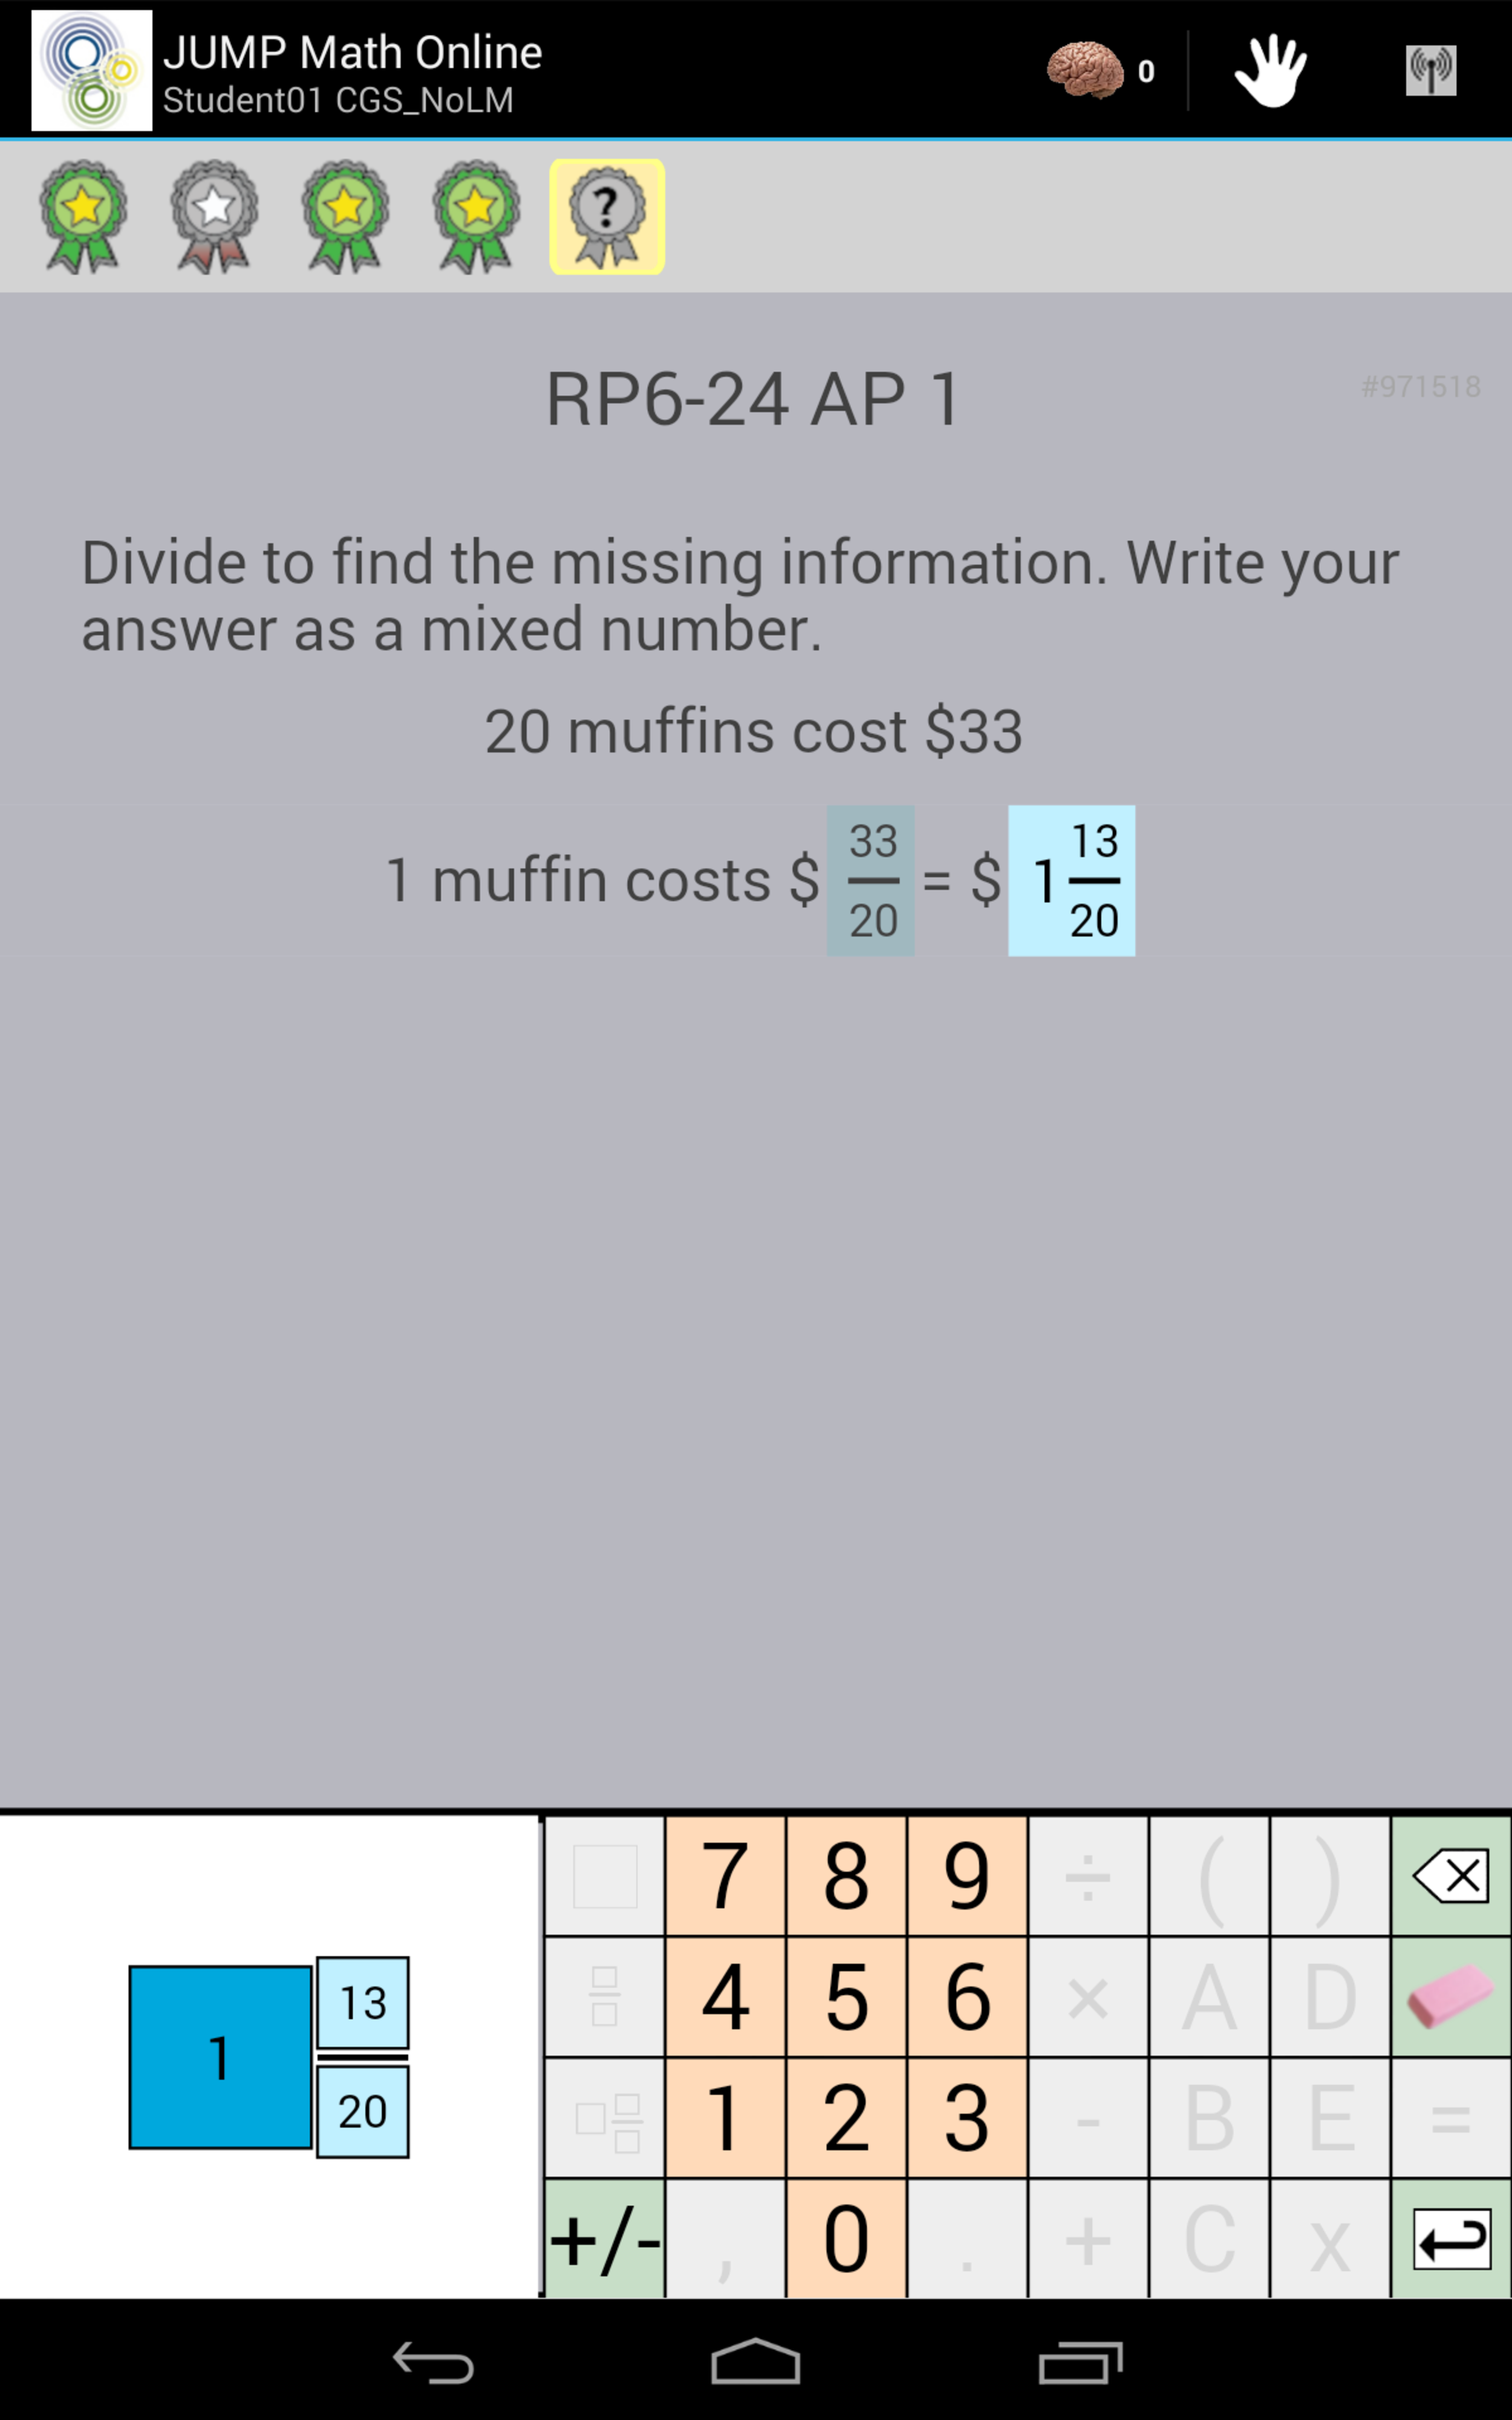
\includegraphics[width=40mm]{images/Student.pdf}}
\caption{
Screenshots of the Teacher and Student software. Figure (a) shows the teacher lesson view. Figure (b) shows a prompt for the teacher to ``Start Exercise 1'' on all student tablets. Figure (c) shows the teacher Dashboard that displays student problem-solving progress. Figure (d) shows the student problem-solving interface, with a calculator input interface at the bottom of the screen and badges at the top that indicate problem correctness. }
\label{fig:Spreadsheet}
\end{figure*}

\section{Method}
We conducted a ten-week study of the software in the fall of 2014 to learn the strengths and weaknesses of the student and teacher software, and to observe the process of integrating a technology-delivered curriculum into real-world classrooms.

%%We conducted a ten-week study of the Enlearn Platform during the fall of 2014. The goal of the the study was to learn about the strengths and weaknesses of the student and teacher software, and to observe the process of integrating a technology-delivered curriculum into real-world classrooms.

%We developed a few experimental hypotheses prior to the trial based on the design goals of the Enlearn software. One of the central design goals was to provide teachers with real-time information about their students to support decision making. We expected teachers with access to this information to re-teach confusing concepts more often, and also to spend more time assisting individual students.
%
%{\bf Hypothesis 1: }\emph{Teachers will re-teach concepts more often in Enlearn classrooms.}
%
%{\bf Hypothesis 2: }\emph{Teachers will assist individual students more often in Enlearn classrooms.}
%
%The other central design goal was to optimize practice problem progressions to meet the needs of individual students. Since students are able to move at their own pace with the tablet-based software, and less classroom management is required, we expected students to solve more problems in the Enlearn classes. We also expected students to learn concepts more effectively and perform better on both the AP problems and the unit post-tests in the tablet-based classes.
%
%{\bf Hypothesis 3: }\emph{Students will complete more Exercise and AP problems in Enlearn classrooms.}
%
%{\bf Hypothesis 4: }\emph{Students will perform better on AP problems and unit post-test in Enlearn classrooms.}
%
%In addition to evaluating these formal hypotheses, our study was designed to capture any interesting trends in the qualitative and quantitative measures collected during the trial to help us gain a complete understanding of the impact of the Enlearn software on student and teacher behavior in the classroom. In the follow sections, we describe our study design and methodology in detail.

\begin{table*}[ht]
\begin{center}
\scriptsize
\begin{tabular}{ | c | c | c | c | c | c | c | c | c | c | c | c | c | c | }
\hline
\bf{School} & \bf{Teaching} & \bf{\# Classes}  & \bf{\# Students}  & \bf{Free Lunch} & \bf{ELL} & \bf{Math Score} & \bf{Reading Score} & \bf{AI/AN}  & \bf{A/PI} & \bf{B}& \bf{H} & \bf{W} & \bf{2+}  \\ \hline
\emph{A} & Co-Taught & 4 & 72 & 10.0\% & 1.9\% & 88.2\% & 90.4\% & 0.4\% & 10.8\% & 2.3\% & 7.1\% & 72.1\% & 7.3\%   \\
\emph{B} & One Teacher & 2 & 39 & 53.0\% & 7.0\% & 55.0\% &  69.5\% & 0.6\% & 16.1\% & 12.1\% & 18.9\% & 37.8\% & 14.4\%   \\ 
\emph{C} & One Teacher & 3 & 63 & 63.6\% & 16.4\% & 56.7\% & 70.3\% & 1.0\% & 27.1\% & 41.3\% & 10.5\% & 11.2\% & 8.9\%   \\
\emph{D} & One Teacher & 2 & 45 & 50.8\% & 5.7\% & 64.0\% & 64.0\% & 2.5\%  & 14.9\% & 14.6\% & 23.4\% & 31.4\% & 13.4\%  \\   \hline
\end{tabular}
\newline
\vspace{0.001in}
\newline
\begin{tabular}{ | l | }
 \hline
{\bf ELL} = English Language Learner, {\bf AI/AN} = American Indian / Alaskan Native,  {\bf A/PI} = Asian / Pacific Islander,  {\bf B} = Black,  {\bf H} = Hispanic,  {\bf W} = White,  {\bf 2+} = Two or More Races.  \\
\hline
\end{tabular}
\end{center}
\vspace{0.04in}
\caption{Data for the four schools.}
\label{fig:Schools}
\end{table*}

\subsection{Participants}
We recruited sixth-grade math teachers from four urban public schools in a northwestern city to participate in our trial. At each school, one teacher (or pair of co-teachers) participated. The teachers taught between two and four sixth-grade math classes, all of which were included in the trial.  A total of 219 students participated in 11 classes. The schools represent a diverse set of communities; one serves a high-income neighborhood, two serve low-income neighborhoods, and one serves a low-income neighborhood but is co-managed by both the state and a non-profit organization. More information about each school is provided in Table \ref{fig:Schools}. We discuss school demographics in detail below. Parents, teachers and school principals gave informed consent for student participation.

%%We recruited sixth-grade math teachers from four urban public schools in a northwestern city to participate in our trial. At each school, one teacher (or pair of co-teachers) participated. The teachers taught between two and four sixth-grade math classes, all of which were included in the trial.  A total of 219 students participated in eleven classes. The schools represent a diverse set of communities; one school serves a high-income neighborhood, two serve low-income neighborhoods, and one serves a low-income neighborhood but is co-managed by both the state and a non-profit organization. More information about each school is provided in Table \ref{fig:Schools}, and we discuss school demographics in detail below. Informed consent for student participation in this study was given by parents, teachers, and school principals.

\subsection{Procedure}
Our study had two conditions: a control condition using the original paper version of the JUMP Math curriculum, and an experimental condition using the tablet-based version. At each school, one class was assigned to the control condition and the remaining classes were assigned to the experimental condition. Since this was a long-term intervention that would strongly impact the dynamics of the participating classes, we allowed teachers to select which classes would receive the tablet-based curriculum. At all four schools, teachers chose to use the tablet-based curriculum with their weaker classes.

None of the teachers had used the JUMP Math curriculum previously, so at the beginning of the trial we conducted a 3-hour curriculum training session for the teachers. During this training, a JUMP Math representative described the curriculum philosophy and walked through example lessons. We also gave teachers separate training to learn the features of the tablet-based software. During the first week of school, we also conducted a  training session for students in each class.

We designed the trial to last for ten weeks and cover four units of the JUMP Math curriculum. While we originally planned to create tablet-based versions of all four units, we were only able to complete units 2 and 4 due to time constraints. As a result, all classes began with a paper version of Unit 1, which was followed by either a paper or tablet version of Unit 2, a paper version of Unit 3, and either a paper or tablet version of Unit 4. Students were given pre- and post-tests designed by JUMP before and after each unit.

%%Our study had two conditions: a control condition in which classes used the original paper version of the JUMP Math curriculum, and an experimental condition in which classes used the tablet-based version of the curriculum. At each school, one class was assigned to the control condition and the remaining classes were assigned to the experimental condition. Since this was a long-term intervention that would strongly impact the dynamics of the participating classes, we allowed teachers to select the classes that would receive the tablet-based curriculum. At all four schools, teachers chose to use the tablet-based curriculum with their weaker classes.
%%
%%None of the teachers had used the JUMP Math curriculum previously, so at the beginning of the trial Enlearn and JUMP Math conducted a 3-hour curriculum training session for the teachers. During this training, a JUMP Math representative described the curriculum philosophy and walked through example lessons. Teachers also had a separate training with Enlearn staff to learn the features of the tablet-based software. During the first week of school, Enlearn also conducted a short training session for students in each of the classes.
%%
%%The trial was designed to last for ten weeks and cover four units of the JUMP Math curriculum. While we originally planned to create tablet-based versions of all four units, we were only able to complete units 2 and 4 due to time constraints. As a result, all classes began with a paper version of Unit 1, which was followed by either a paper or tablet version of Unit 2, a paper version of Unit 3, and either a paper or tablet version of Unit 4. Students were given pre- and post-tests designed by JUMP before and after each unit.

\subsection{Measures}
Our study has a mixed design with both qualitative and quantitative measures. Our qualitative measures captured high-level feedback on the Enlearn Platform from participating teachers as well as the impressions of staff from the non-profit who spent extensive time observing teachers in the classroom. Our quantitative measures captured information about teacher behavior in the classroom, student problem-solving behavior, and student engagement. We discuss each measure in detail and present results in the following sections.

\begin{table}
\begin{center}
\scriptsize
\begin{tabular}{ | c | c | c | c | c | c | c | c | c | c | c | c | c | c | }
\hline
\bf{School} & \bf{Quality} & \bf{Org.} & \bf{Support} & \bf{Prep.}  & \bf{Rapport}  & \bf{Challenges}  \\ \hline
\emph{A} & 4 & 4 & 4.33 & 4.33 & 4.33 & 1.67 \\
\emph{B} & 1.33 & 1 & 1.5 & 2 & 2.33 &  3.67 \\ 
\emph{C} & 3 & 3 & 1.67 & 3.25 & 4.25 & 4.75 \\ 
\emph{D} & 4.75 & 5 & 4.5 & 5 & 4.5 & 2.75 \\ \hline
\end{tabular}
\newline
\vspace{0.001in}
\newline
\begin{tabular}{ | l | }
\end{tabular}
\end{center}
\vspace{0.04in}
\caption{Results for the Likert-scale questions of our survey of Enlearn classroom observers. For each school, we collected data on the overall quality of the teacher, the level of class organization, the level of support provided by school administrators, the level of teacher preparedness, the rapport between teachers and students, and the level of challenge presented by students (issues at home, English language learners, etc).}
\label{fig:Ratings}
\end{table}

\section{School Characterization}
The schools that we worked with in this study serve diverse communities and the teachers and students at each school face a different set of daily challenges. School demographic factors alone do not capture the environment at each school; teacher behavior, classroom dynamics, and other social factors also have a strong impact. Extensive research in education shows that teachers greatly influence student behavior and achievement \cite{Hill2005, Wentzel2002, Reeve2004, Wright1997}. As a result, we were interested in viewing the process of integrating a technology-delivered curriculum in each school through the lens of the specific classroom and teacher environment. 

To capture qualitative information about each classroom, we conducted a survey of the four staff members of hte non-profit who spent time in all four schools. These staff members observed and supported teachers weekly throughout the trial. The survey included both Likert-scale questions and free-form questions. The questions focused on quality of teacher instruction, level of support principals provide for teachers, and level of challenge presented by students (issues at home, English language, stress). Table \ref{fig:Ratings} shows results of the Likert-scale questions and Table \ref{fig:Schools} show school demographic data. Below, we discuss the dynamics at each of the four schools, which we refer to as Schools A, B, C and D.

%%To capture qualitative information about each classroom, we conducted a survey of the four Enlearn staff members who spent time in all four schools. These staff members observed teachers weekly throughout the trial, and served as support for teachers. The survey included both Likert-scale questions and free-form questions. The questions focused on the quality of teacher instruction, the level of support principals provide for teachers, and the level of challenge presented by students (issues at home, English language, stress). The results of the Likert-scale questions are shown in Table \ref{fig:Ratings} and data on school demographics are shown in Table \ref{fig:Schools}. We discuss the dynamics at each of the four schools, which we refer to as Schools A, B, C and D, in turn below.

\subsection{School A}
This school serves a high-income, predominantly white neighborhood. Two teachers co-taught, leading lessons in turn. Observers reported that both teachers were prepared, kept the classroom organized, and supported each other effectively. They had a strong grasp on lesson content, and changed teaching tactics throughout the day if a particular approach was not effective. One observer noted that ``\emph{the teachers have a strong rapport with the students, leading to greater connection and willingness to pursue help during free periods and even lunch time.}" Students were generally well behaved, with little need for disciplinary intervention. Although a few students had behavioral or learning challenges, they often had personal aides. Teachers were well-supported by the school's principal, who visited classes occasionally.

%%This school serves a high-income, predominantly white neighborhood. The classes were co-taught by two teachers who took turns leading lessons. Observers reported that both teachers were prepared, and that they keep the classroom organized and supported each other effectively. They had a strong grasp on lesson content, and changed teaching tactics throughout the day if a particular approach was not effective. One observer noted that ``\emph{the teachers have a strong rapport with the students, leading to greater connection and willingness to pursue help during free periods and even lunch time.}" Students were generally well behaved, with little need for disciplinary intervention, and although a few students had behavioral or learning challenges, they often had personal aides. Teachers were well-supported by the school's principal, who visited classes occasionally.

%This school serves a high-income neighborhood. The classes were co-taught by two teachers, who took turns delivering lesson material. Observers reported that both teachers were prepared, kept the classroom well organized and supported each other effectively. They had a strong grasp on lesson material and would change lesson tactics throughout the day if it appeared a particular approach was not working. One observer noted, "the teachers have a strong rapport with the students, leading to greater connection and willingness to pursue help during free periods and even lunch time." The teachers encouraged students to put in effort regardless of correct answer. The school's principal visited classes occasionally. Students were generally well behaved, with little need for disciplinary intervention. Although a few students had behavioral or learning challenges, they often had personal aides who also helped other nearby students.

\subsection{School B}
This school serves a racially diverse, low-income neighborhood. Observers reported that this teacher was ineffective and unable to restore order once students started to go off-task. The classroom was disorganized, and the teacher seemed inattentive. One observer noted that ``\emph{on every count, the instruction was weak.}'' Although the teacher and students seemed to get along, his disciplinary approach did not work; consequently, both teacher and students would often raise their voices to draw attention, resulting in a chaotic learning environment. The students faced a moderate amount of home challenges, with a significant portion of students also being English Language Learners (ELL), but external help was not present. The teacher did not effectively support students in figuring out how to be more engaged. Likewise, he did not receive support or feedback to improve his teaching.

%%This school serves a racially diverse low-income neighborhood. Observers reported that this teacher was ineffective and unable to restore order once students started to go off-task. The classroom was disorganized, and the teacher seemed inattentive. One observer noted that ``\emph{on every count, the instruction was weak.}'' Although the teacher and students seemed to get along, the teacher's disciplinary approach did not work; consequently, both teacher and students would often raise their voices to draw attention, resulting in a chaotic learning environment. The students faced a moderate amount of home challenges, with a significant portion of students also being English Language Learners (ELL), but external help was not present. The teacher did not effectively support students in figuring out how to be more engaged. Likewise, he did not receive support from administrators or feedback to improve his teaching.

\subsection{School C}
This school serves a racially diverse low-income neighborhood. The teacher was typically prepared for class, although``\emph{not ready to teach in any engaging way.}" Call-and-response or fill-in-the-blank teaching was common, which failed to retain some students' focus. However, the teacher was liked and respected by students. The students at this school presented many challenges; ``\emph{most of them have some sort of trauma that they are dealing with}'' such as homelessness, unstable home environments, trauma and language barriers. Despite these issues, the school only offered a part-time counselor. Observers reported that the principal was rarely on campus, and teachers saw her as``\emph{having abandoned the children.}" Classroom activities were often disrupted by last minute events like school assemblies and schedule changes. Overall, the classroom environment was erratic, but the teacher had a strong handle on managing her students.

%This school serves a racially diverse low-income neighborhood. The teacher was usually prepared for class, though, an observer noted, "not ready to teach in any engaging way." Another observer mentioned that she would often ask a question, then wait for a response (or answer the question if no one responded), which led to some students losing focus as they knew they would not be called on to participate. There were a few aides who supported students with special needs, but did not contribute to classroom management. Observers reported that the principal was rarely on campus, and teachers saw her as "having abandoned the children". Classroom activities were often disrupted by last minute events like school assemblies and schedule changes. The teacher was liked and respected by the students, and she would advise them on topics unrelated to math as well. The students' personal issues caused challenges for instruction, though. Many students faced stresses like homelessness, unstable home environments, trauma and language barriers. Despite these issues, the school only offered a part-time counselor. The classroom environment was erratic, with students constantly causing interruptions, but the teacher had a relatively strong handle on managing her students.

\subsection{School D}
This school serves a racially diverse low-income neighborhood, but is co-managed by the state and a non-profit organization with a STEM-education focus. The teacher was highly prepared, providing strong support and high quality instruction. The classroom was``\emph{unbelievably organized,}'' with students obedient at all times while still having fun. One observer said that ``\emph{students would rush to do whatever she asked.}" This may have been a result of training held for students at the beginning of the year on staying focused in class. Students showed respect, and the teacher reciprocated. The school principal dropped by occasionally, and the teacher kept in regular contact with both the principal and technology lead of the school. Although many students came from immigrant families and faced some home challenges, there were no obvious signs of issues based on the effective classroom management. One observer noted that since this was a specially funded school, the students likely had families who were invested enough in education to enroll their children.

%%This school serves a racially diverse low-income neighborhood, but is co-managed by the state and a non-profit organization with a STEM-education focus. The teacher was highly prepared, providing strong support and high quality instruction, with a firm grasp of both the material and each day's lesson plan. The classroom was``\emph{unbelievably organized.}'' Another observer described it as ``\emph{very controlled,}'' with students obedient at all times while still having fun. One that ``\emph{students would rush to do whatever she asked.}" This may have been a result of a teacher training held at the beginning of the year on helping students stay focused during class. Students showed respect, and the teacher reciprocated. The school principal dropped by occasionally, and the teacher kept in regular contact with both the principal and technology lead of the school. Although many students came from immigrant families and faced some home challenges, there were no obvious signs of issues, based on the effective classroom management. One observer noted that since this was specially funded school, the students likely had families who were invested enough in education to enroll their children.


%\begin{table}
%\begin{center}
%\scriptsize
%\begin{tabular}{ | c | c | c | c | c | c | c | c | c | c | c | c | c | c | }
%\hline
%\bf{School} & \bf{Progress} & \bf{Group Teaching} & \bf{Individual Teaching} & \bf{Independence} & \bf{Behavior}  & \bf{Learning}  \\ \hline
%\emph{A1} & 4 & 4 & 4 & 4 & 2 & 3 \\
%\emph{A2} & 4 & 2 & 2 & 2 & 2 & 2 \\
%\emph{B} & 3 & 3 & 4 & 3 & 3 & 3 \\ 
%\emph{C} & 4 & 3 & 3 & 3 & 3 & 3\\ 
%\emph{D} & 4 & 3 & 3 & 4 & 3 & 3\\ \hline
%%\emph{A1} & Extremely & Extremely& Extremely & Extremely & Somewhat & Very much \\
%%\emph{A2} & Extremely & Somewhat & Somewhat & Somewhat & Somewhat & Somewhat \\
%%\emph{B} & Very much & Very much & Extremely & Very much & Very much & Very much \\ 
%%\emph{C} & Extremely & Very much & Very much & Very much & Very much & Very much\\ 
%%\emph{D} & Extremely & Very much & Very much & Extremely & Very much & Very much\\ \hline
%\end{tabular}
%\newline
%\vspace{0.001in}
%\newline
%\begin{tabular}{ | l | }
%\end{tabular}
%\end{center}
%\vspace{0.04in}
%\caption{Results for the Likert-scale questions (scale from 1-4) from our survey of teachers who participated in the trial. From each teacher, we collected data on whether using the tablet enhanced their ability to monitor student progress during class, led them to adjust teaching strategy and instructional approach for whole group lessons and individual students, increased student independent work rate, supported positive behaviors related to classroom management, and enhanced student learning compared to teaching with paper lessons}
%\label{fig:TeacherSurvey}
%\end{table}

\section{Findings: Teacher Surveys}
At the end of the study, we asked each teacher to complete a survey about their experiences with our tablet-based software. The survey included both Likert-scale and free-form questions. The questions focused on strengths and weaknesses of the Enlearn software and the most positive and negative changes caused by introducing the software into classrooms.

Overall, teachers viewed the software positively; all responded that they would recommend the software to a colleague. They felt that students were more motivated, engaged and focused when using the tablets. Teachers noted that ``\emph{students were catching their misunderstandings quickly and asking for help}", and students were ``\emph{accountable for their learning, which...seemed to make them more receptive to receiving help}". These responses suggest that students were assisted by the real-time feedback provided by the tablet software, and that this gave them a sense of ownership over their learning.

The software also helped teachers to monitor individual student understanding. ``\emph{It was very easy to see what kids were struggling with the problems}," said one teacher. Another said ``\emph{It is a great way to see how EVERY student is doing.}''  While providing individual assistance to particular students, the tablets kept other students on task. On the professional development side, one teacher answered, ``\emph{We learned a lot about our teaching practice, as well as how our students function to try and hide misconceptions and struggles in math}."

While the real-time data provided to students and teachers was effective, teachers also suggested some ways to improve the student software. One noted that ``\emph{the fill-in-the-blanks aspect seemed to prevent students from making important connections when building on concepts. I think a stylus would help with entering the answers, and would eliminate the frustration that students felt with the way they currently have to input their answers.}'' Another noted that ``\emph{a few students would just mash random answers in an attempt to see how many problems they could do}.''  To help monitor student progress, another suggested adding a feature to the Dashboard ``\emph{to show if students got the problem wrong initially, then went back to change it to the correct answer}.

Another common concern was that the tablet was not locked, so students would sometimes go off-task to play with other apps or settings. One of the teachers at School A, which serves a high-income neighborhood, commented that since most of their students had personal electronic devices, they would often approach the exercises as if ``\emph{playing a game on their phone}". The teacher from School D, which is co-managed by a STEM-focused non-profit, also noted that some students were distracted by other apps and features because the tablets felt novel in contrast to other classroom technologies that were used more frequently.

Overall, teachers and students appeared to benefit from the availability of real-time data and feedback. While there are some important areas for future design iteration, the introduction of a tablet-based curriculum into the classroom did not appear to disrupt the classroom workflow.

\begin{figure*}[t]
\centering
\subfigure[]{\label{fig:Assists}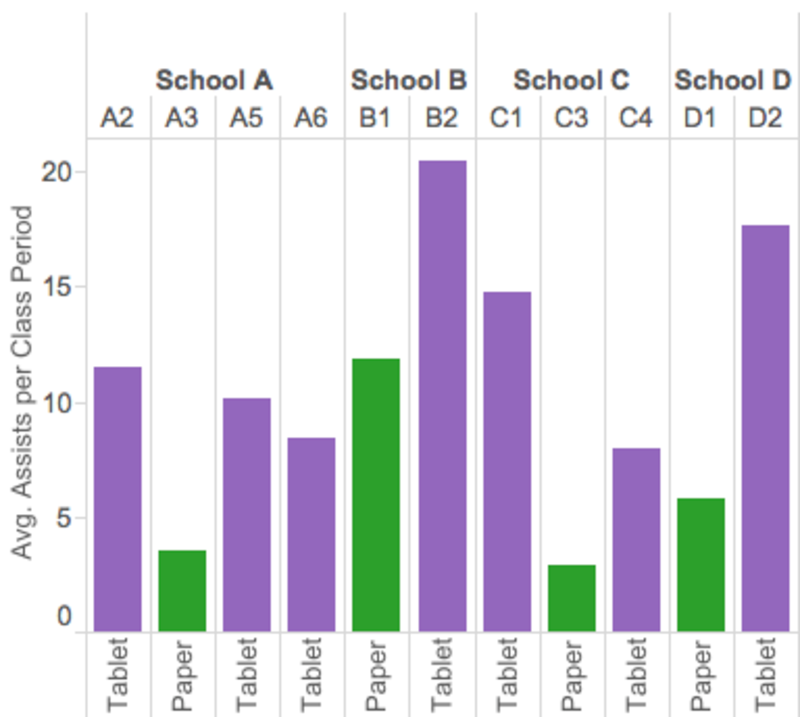
\includegraphics[height=40mm]{images/assists.pdf}} \hspace{0.5em}%
\subfigure[]{\label{fig:Reteaches}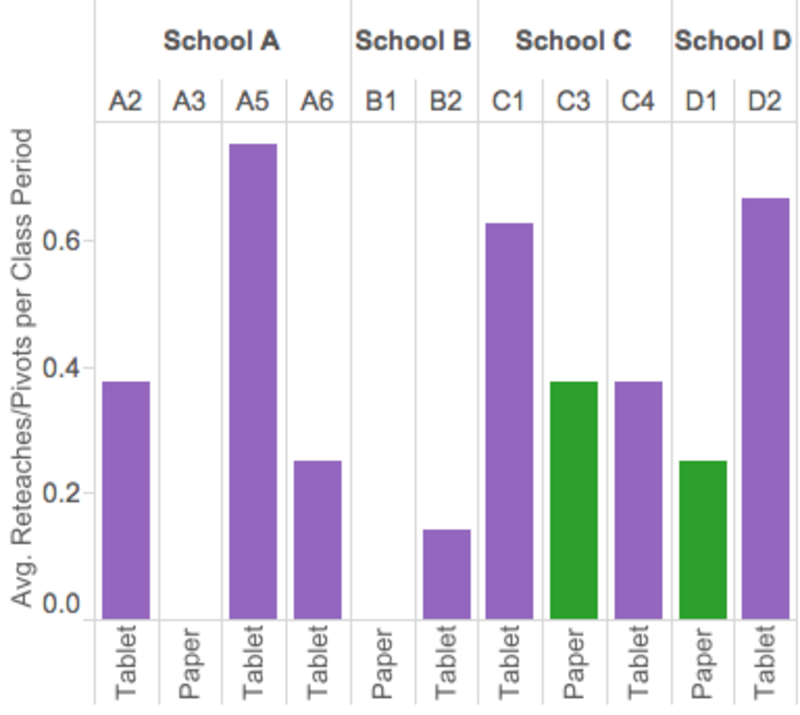
\includegraphics[height=40mm]{images/reteach.pdf}} \hspace{0.5em}%
\subfigure[]{\label{fig:ClassTime}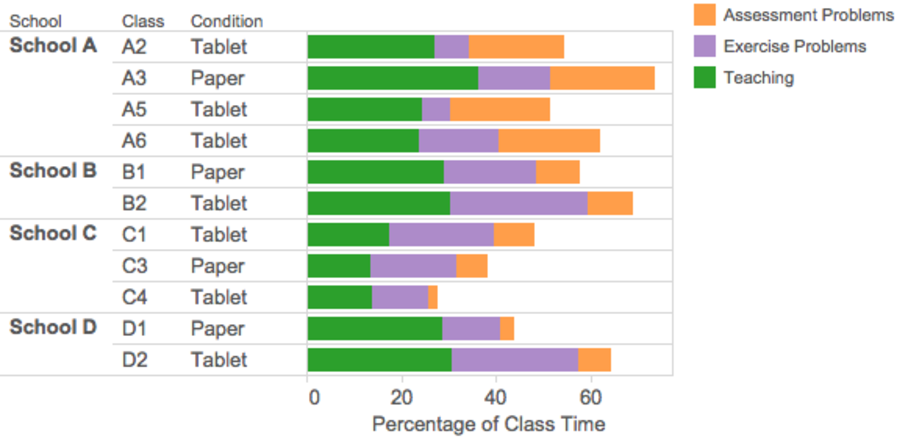
\includegraphics[height=40mm]{images/taplog.pdf}} \hspace{0.5em}%
\caption{
Figure (a) shows the average number of assists per class period, broken down by school and class. Figure (b) shows the average number of reteaches and pivots per class period, broken down by school and class. Figure (c) shows a breakdown of the percentage of time teachers spent on assessment problems, exercise problems, and teaching.}
\label{fig:Spreadsheet}
\end{figure*}

\section{Findings: Teacher and Student Behavior}
In this section, we present results from statistical analyses of a set of quantitative measures that capture teacher behavior, student problem-solving behavior, and student engagement during the study. For each outcome measure, we are primarily interested in analyzing differences based on \emph{Condition} (either tablet or paper). However, since the schools included in our study are substantially different from each other, we also analyzed differences based on the covariate \emph{School}. Finally, we expect that the tablet-based intervention may have different effects at different schools, so we analyzes the interaction between \emph{Condition} and \emph{School} to capture these differences.

Before analyzing our continuous outcome measures, we evaluated the Shapiro-Wilk test to assess the normality of our data, and found that it was statistically significant for all of our measures, meaning none of them were normally distributed. As a result, we applied the Aligned Rank Transform \cite{Higgins94, Salter93} procedure on each of our continuous outcome measures. This procedure aligns and ranks non-parametric data so that a standard ANOVA model can be used to perform a factorial analysis. For each main effect or interaction, the ART procedure aligns the data such that only that main effect or interaction remains, and then ranks the aligned data. A standard ANOVA model can then be used on the ranked data to measure the effect for which it was aligned. We used the ARTool program to align and rank our data \cite{Wobbrock11}.

In the cases where there is a significant \emph{Condition*School} interaction, we perform a follow-up analysis for each school to determine how the outcome measure differs based on \emph{Condition} at that school. For these comparisons, we use a Kruskal Wallis test to analyze our continuous outcome measures. Since this produces a large number of statistical comparisons, we risk inflating alpha. To address this potential issue, we sum \emph{p}-values across all comparisons for each outcome measure to ensure that the combined alpha still falls below the 0.05 threshold. We also report effect sizes in addition to \emph{p}-values to show the magnitude of the differences between our populations. We use an Eta-Squared ($\eta^2$) measure of effect size for our factorial analyses and an \emph{r} measure of effect size for analyses within schools. For $\eta^2$, effects with values of 0.01 are \emph{small}, 0.06 are \emph{moderate}, and 0.14 or greater are \emph{large}. For \emph{r}, effects with values of 0.1 are \emph{small}, 0.3 are \emph{moderate}, and 0.5 or greater are \emph{large}.



\subsection{Teacher Behavior Changes With Access to Data}
In addition to our surveys of the teachers experiences working with the our platform, we wanted to study how their behavior differed in the tablet and paper classes. We expected teacher to be impacted by the availability of real-time student data, and would spend more time re-teaching concepts and assisting individual students as a result. We also wanted to study how teachers chose to spend class time in each type of class, and whether tablets influenced classroom activities.

To compare teacher behavior in the two types of classes, we observed teachers regularly throughout the study, a total of 8 observation days per class. We developed a tablet application for logging teacher observations called the ``Teacher Taplog.'' This application provides buttons that the observer can press to log the current classroom activity, such as ``Teaching,'' ``Demo,'' or ``AP Problems.'' Actions that occur during a classroom activity, such as ``Assisting Student,'' can also be logged. All observers were staff members at the non-profit organization that we partnered with, and all were trained in advance and tested for inter-rater reliability.
%We tried to schedule observation days at regular intervals in each school, but this was difficult due to teacher constraints. The observation dates for each school are given in Table \ref{fig:ObservationDays}.

In our analysis of the Teacher Taplog data, we treat each class as a subject in our experiment. For each outcome measure, such as the time spent on teaching, we aggregate across all observation days to calculate the average amount of time spent teaching during that class period. While we have relative rich data about how the teacher spent time during each class, we only have a total of eleven classes in our study, which is a small number for statistical analysis. As a result, we are unlikely to see significant effects for many of our measures.

\subsubsection{Number of Student Assists}
Using the Teacher Taplog, our observers recorded each time a teacher assisted an individual student and the duration of the assist. We analyzed the average amount of time that teachers spend assisting students, and while \emph{Condition} did not have a significant effect, there was a trend towards teachers assisting students more in the tablet classes (F(1,3)=8.459, \emph{p}=0.0621). Neither \emph{School} (F(3,3)=1.462, \emph{n.s.}) nor the \emph{Condition*School} interaction (F(3,3)=0.131, \emph{n.s.}) had a significant effect on assist time. We also analyzed the average number of times teachers assisted students. Again, \emph{Condition} did not have a significant main effect, but there was a trend toward teachers assisting students more often in the tablet-based classes (F(1,3)=7.493, \emph{p}=0.0715). Neither \emph{School} (F(3,3)=1.652, \emph{n.s.}) nor the \emph{Condition*School} interaction (F(3,3)=0.283, \emph{n.s.}) had a significant effect on number of student assists. 

Figure \ref{fig:Assists} shows the average number of assists for each of the eleven classes. The visualization clearly suggests that teachers assist students more often in the tablet classes. This suggests that teachers respond to the real-time student data, a finding that is supported by the results of the teacher survey. Teachers reported that the software helped them identify struggling students and encouraged students to ask for help.



\subsubsection{Number of Re-Teach Events}
A ``re-teach'' event is when a teacher stops the class to clarify a concept or present it in a new way. Our observers were trained to recognize and log re-teach events using the Teacher Taplog. While our analysis showed that emph{Condition} did not have a significant effect on re-teaches, there was a trend towards more re-teach events in the tablet classes (F(1,3)=8.459,\emph{p}=0.0621). Neither \emph{School} (F(3,3)=1.131, \emph{n.s.} nor the \emph{Condition*School} interaction (F(3,3)=0.444, \emph{n.s.}) had a significant effect on the number of re-teach events.

Figure \ref{fig:Reteaches} shows the average number of re-teach events during each class. The data show that re-teaches happen very infrequently, less than once per class, but that teachers are re-teaching more often in the tablet classes. This suggests that teachers are using real-time student data to determine when students are struggling and need additional teaching on a concept, an observation that mirrors teacher survey comments.


%\begin{figure}[t]
%\centering
%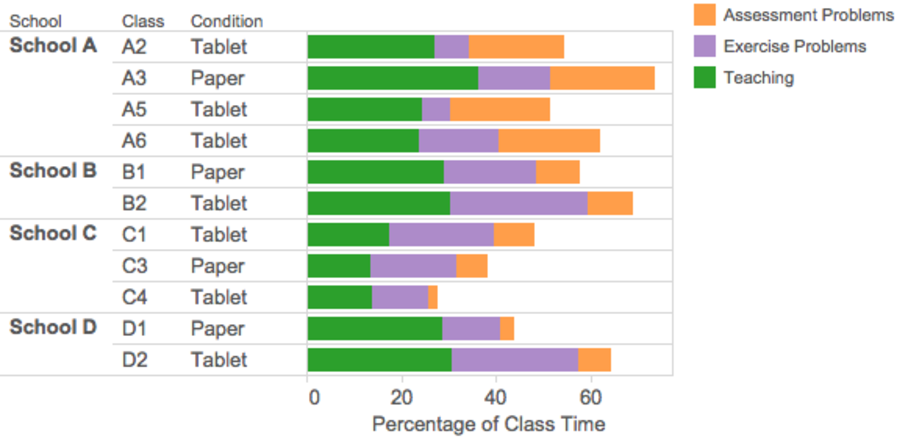
\includegraphics[width=90mm]{images/taplog.pdf}
%\caption{The average percentage of total class time spent on teaching, exercise problems, and Assessment (AP) problems in each classroom.}
%\label{fig:ClassTime}
%%\vspace{-0.04in}
%\end{figure}

\begin{table*}[!htb]
\begin{center}
%%
%% NOTE: this file is generated by a script!
%% You should not edit this file directly, but instead edit data_table.py and regenerate this file.
%%

\small
\begin{tabular}{|c|c|c|ccc|ccc|c|c|c|}
\hline
School & Unit & Condition& \multicolumn{3}{|c|}{\# Exercise Problems} & \multicolumn{3}{|c|}{\# AP Problems} & \% AP Correct & \% Pre-Test & \% Post-Test\\
\hline
\hline
\multirow{4}{*}{A}  & 
\multirow{2}{*}{Unit 2}  & 
Tablet & 51.5 & \scriptsize{$N=70$} & \scriptsize{$p<0.05$} & 351.5 & \scriptsize{$N=70$} & \scriptsize{$p<0.005$} & 97.95\% & 33\% & 56\%  \\
 & 
 & 
Paper & 77.5& \scriptsize{$Z=2.181$} & \scriptsize{$r=0.26$} & 399.5 & \scriptsize{$Z=3.076$} & \scriptsize{$r=0.37$} & 92.18\% & 35\% & 53\%    \\
\cline{2-12}
 & 
\multirow{2}{*}{Unit 4}  & 
Tablet & 334.8 & \scriptsize{$N=72$} & \scriptsize{$p<0.001$} & 277.5 & \scriptsize{$N=72$} & \scriptsize{$p<0.005$} & 98.39\% & 45\% & 73\% \\
 & 
 & 
Paper & 149.5 & \scriptsize{$Z=-5.587$} & \scriptsize{$r=0.66$} & 245 & \scriptsize{$Z=-3.251$} & \scriptsize{$r=0.38$} & 87.84\% & 45\% & 81\% \\
\hline
\hline
\multirow{4}{*}{B}  & 
\multirow{2}{*}{Unit 2}  & 
Tablet & 669 & \scriptsize{$N=39$} & \scriptsize{$p<0.001$} & 70.5 & \scriptsize{$N=39$} & \scriptsize{$p<0.05$} & 88.46\% & 13\% & 35\%   \\
 & 
 & 
Paper & 284 & \scriptsize{$Z=5.041$} & \scriptsize{$r=0.81$} & 97.25 & \scriptsize{$Z=-2.478$} & \scriptsize{$r=0.40$} & 79.45\% & 33\% & 43\%    \\
\cline{2-12}
 & 
\multirow{2}{*}{Unit 4}  & 
Tablet & 257 & \scriptsize{$N=39$} & \scriptsize{$p<0.001$} & 89 & \scriptsize{$N=39$} & \scriptsize{$n.s.$} & 88.46\% & 9\% & 22\% \\
 & 
 & 
Paper & 26 & \scriptsize{$Z=5.115$} & \scriptsize{$r=0.82$} & 89.5 & \scriptsize{$Z=-0.397$} &  & 75.36\% & 27\% & 45\% \\
\hline
\hline
\multirow{4}{*}{C}  & 
\multirow{2}{*}{Unit 2}  & 
Tablet & 503 & \scriptsize{$N=63$} & \scriptsize{$p<0.001$} & 230 & \scriptsize{$N=63$} & \scriptsize{$p<0.001$} & 95.29\% & 50\% & 60\%  \\
 & 
 & 
Paper & 157 & \scriptsize{$Z=-6.342$} & \scriptsize{$r=0.80$} & 440 & \scriptsize{$Z=5.552$} & \scriptsize{$r=0.70$} & 85.69\% & 40\% & 47\%   \\
\cline{2-12}
 & 
\multirow{2}{*}{Unit 4}  & 
Tablet & 411 & \scriptsize{$N=63$} & \scriptsize{$p<0.001$} & 206 & \scriptsize{$N=63$} & \scriptsize{$p<0.005$} & 97.24\% & 45\% & 68\% \\
 & 
 & 
Paper & 66.5 & \scriptsize{$Z=-6.342$} & \scriptsize{$r=0.80$} & 246.5 & \scriptsize{$Z=3.256$} & \scriptsize{$r=0.41$} & 89.96\% & 59\% & 82\% \\
\hline
\hline
\multirow{4}{*}{D}  & 
\multirow{2}{*}{Unit 2}  & 
Tablet & 686.5 & \scriptsize{$N=45$} & \scriptsize{$p<0.001$} & 236 & \scriptsize{$N=45$} & \scriptsize{$n.s.$} & 97.07\% & 35\% & 48\% \\
 & 
 & 
Paper & 347 & \scriptsize{$Z=5.733$} & \scriptsize{$r=0.85$} & 262 & \scriptsize{$Z=-1.124$} &  & 89.29\%  & 40\% & 46\% \\
\cline{2-12}
 & 
\multirow{2}{*}{Unit 4}  & 
Tablet & 847.5 & \scriptsize{$N=45$} & \scriptsize{$p<0.001$} & 126 & \scriptsize{$N=45$} & \scriptsize{$p<0.05$} & 95.76\% & 36\% & 84\% \\
 & 
 & 
Paper & 226 & \scriptsize{$Z=5.734$} & \scriptsize{$r=0.86$} & 165 & \scriptsize{$Z=-2.124$} & \scriptsize{$r=0.32$} & 85.94\% & 36\% &90\% \\
\hline
\end{tabular}

\end{center}
\vspace{0.05in}
\caption{\label{tab:ProblemSolvingStats} Results of the comparisons within each school. For each analysis, we show the median values to the left of the cell, along with results of the statistical tests. We also report median percent of AP problems correct and median scores on the unit pre- and post-tests for each school.}
\end{table*}

\begin{figure}[t]
\centering
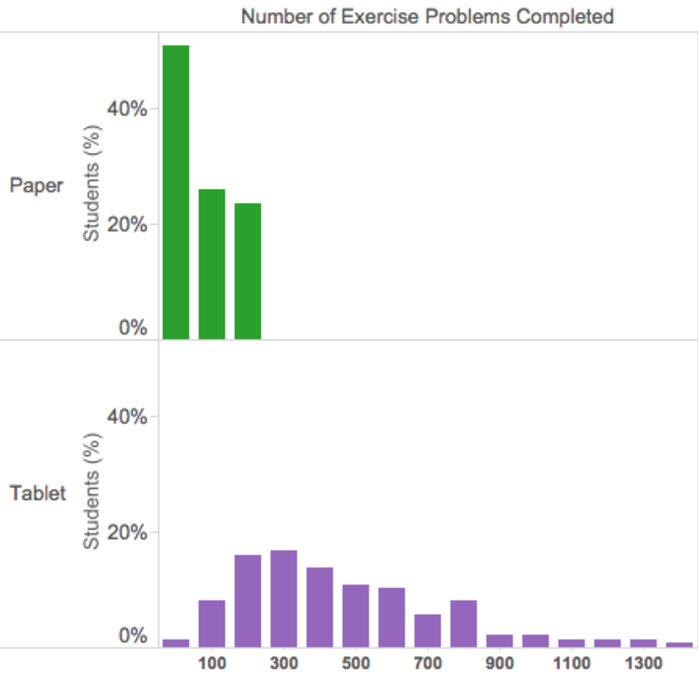
\includegraphics[width=65mm]{images/exercise_histogram.pdf}
\caption{Histogram of exercise problem completion for Unit 4. Each bar represents the percentage of students who fall into the related bin.}
\label{fig:ProblemSolvingEX}
%\vspace{-0.04in}
\end{figure}


\subsubsection{Class Time Usage}
In addition to studying specific classroom behaviors that we expected to change as a result of introducing real-time student data, we also wanted to study how teachers used their time in the tablet and paper classes. In particular, we thought that the time spent teaching and on exercise and AP problems might be influenced by the introduction of tablets. To evaluate this question, we first analyzed the average time spent teaching during each class. We found that \emph{Condition} did not have a significant effect, but there was a trend towards spending less time teaching in tablet classes (F(1,3)=7.493, \emph{p}=0.0715). \emph{School} also had no significant effect, but we measured a trend toward teachers at Schools B and D spending more time teaching than those at Schools A and C F(3,3)=7.248, \emph{p}=0.0690). There was no significant \emph{Condition*School} interaction. We also analyzed the amount of time spent on exercise and AP problems, but found no significant differences based on \emph{Condition}, \emph{School}, or their interaction. 

Figure \ref{fig:ClassTime} shows the average amount of time spent on teaching, exercise problems, and AP problems in each class. While we thought the tablet-delivered curriculum might strongly impact how teacher spend class time, especially problem-solving time since problems were delivered to students through tablets, but this expectation was not substantiated. We did see a trend towards teachers spending less time on teaching in the tablet-based classes, which could be an indication that more time was spent on other activities such as assisting students or classroom management. 
%However, it is clear that the introduction of a tablet-delivered curriculum did not dramatically change how teachers chose to spend class time or disrupt established workflows.

%{\bf Teaching}
%Condition = (F(1,3)=7.493, \emph{p}=0.0715)
%School = (F(3,3)=7.248, \emph{p}=0.0690)
%Condition*School = (F(3,3)=0.145, \emph{n.s.})
%
%{\bf Exercise}
%Condition = (F(1,3)=0.180, \emph{n.s.})
%School = (F(3,3)=2.835, \emph{n.s.})
%Condition*School = (F(3,3)=0.877, \emph{n.s.})
%
%{\bf AP}
%Condition = (F(1,3)=1.759, \emph{n.s.})
%School = (F(3,3)=2.993, \emph{n.s.})
%Condition*School = (F(3,3)=0.629, \emph{n.s.})

\subsection{Student Problem-Solving Behavior is Impacted by Tablets}
We expected student problem-solving behavior to differ in the paper and tablet classes. We hypothesized that the adaptive, self-paced problem progressions would allow students to complete more Exercise and AP problems in the tablet classes, and that students would perform better on the AP problems and unit post-tests. To study problem-solving behavior, we recorded two measures: the number of problems completed, and problem correctness. In the tablet classes, we logged student interactions with the tablet to capture these measures. In the paper classes, we counted and graded AP problems, and counted Exercise problems. The AP problems were clearly labeled in the JUMP AP notebook, but exercise problems were completed in students' personal notebooks, making them difficult to interpret and grade. To count Exercise problems, graders used a well-organized notebook from each class as a template for counting the rest of the notebooks. 

We analyze problem-solving behavior for Units 2 and 4 separately. The units cover different content that could influence problem-solving behavior, and the teachers at Schools B and C ran out of time for Unit 4 and rushed some of the content. As a result, we treat these units separately in the analysis.



\subsubsection{Number of Exercise Problems Completed}
We analyzed the number of exercise problems completed, and found that \emph{Condition} had a significant main effect in both Unit 2 (F(1,209)=141.669, \emph{p}\textless0.0001, $\eta^2$=0.77) and Unit 4 (F(1,211)=373.031, \emph{p}\textless0.0001, $\eta^2$=0.90), with students completing more exercise problems in the tablet classes. \emph{School} also had a significant main effect in both Unit 2 (F(3,209)=160.007, \emph{p}\textless0.0001, $\eta^2$=0.74) and Unit 4 (F(3,211)=53.950, \emph{p}\textless0.0001, $\eta^2$=0.95). Finally, the \emph{Condition*School} interaction had a significant effect in both Unit 2 (F(3,209)=62.511, \emph{p}\textless0.0001, $\eta^2$=0.66) and Unit 4 (F(3,211)=22.971, \emph{p}\textless0.0001, $\eta^2$=0.74), suggesting that tablets had a different effects in different schools.

To understand the effect of \emph{Condition} at each school, we ran a series of follow-up analyses. The results are shown in Table \ref{tab:ProblemSolvingStats}. Students in the tablet classes at Schools B, C, and D complete a huge number of exercise problems, significantly more than those in the paper classes. However, at School A, students in the paper class complete significantly more problems during Unit 2. This trend is reversed in Unit 4; however the Unit 4 effect size is smaller, perhaps because School A spent less time on the exercise problems than the other schools.

The histograms in Figure \ref{fig:ProblemSolvingEX} show that while students completed more exercise problems in the tablet classes on average, there was a large amount of variation. There is much less variation in the paper classes, where students completed exercise problems in lock-step. This shows the potential benefit of generative adaptivity: students can work through problems at their own pace, practicing basic concepts or advancing to more challenging concepts as needed.

%There are also a number of differences between schools. Students at school D completed many more problems than at the other three schools. 

%Schools B and C also completed many fewer exercise problems during Unit 4, which we would expect since both teachers were rushed at the end of the study. The two schools' rushed pace may have been a consequence of their individual teacher and environmental factors - Enlearn observers reported that School B's teacher was very weak, and School C's teacher had to deal with last minute scheduling issues; both teachers received little external support.




\subsubsection{Number of AP Problems Completed}
We also analyzed the number of AP problems completed. We found that \emph{Condition} had a significant effect in both Unit 2 (F(1,209)=41.296, \emph{p}\textless0.0001, $\eta^2$=0.92) and Unit 4 (F(1,211)=14.500, \emph{p}\textless0.0005, $\eta^2$=0.74), and that overall students completed \emph{fewer} AP problems in the tablet classes.\ emph{School} also had a significant effect in both Unit 2 (F(3,209)=50.775, \emph{p}\textless0.0001, $\eta^2$=0.90) and Unit 4 (F(3,211)=106.607, \emph{p}\textless0.0001, $\eta^2$=0.85). Finally, the \emph{Condition*School} interaction had a significant effect in both Unit 2 (F(3,209)=20.880, \emph{p}\textless0.0001, $\eta^2$=0.73) and Unit 4 (F(3,211)=9.527, \emph{p}\textless0.0001, $\eta^2$=0.46), again suggesting that tablets had different effects in different schools.

We ran follow-up analyses at each school, and the results are shown in Table \ref{tab:ProblemSolvingStats}. At School A, students in the paper class completed more AP problems in Unit 2, while students in the tablet class completed more in Unit 4, mirroring the results for exercise problems. However, at Schools B, C, and D, students in the paper classes completed either the same number of AP problems or more than those in the tablet classes. 

These results are surprising. Our analysis of the Teacher Taplog data shows that there is no difference in the amount of time teachers spent on AP problems based on \emph{Condition}. However, at Schools B, C, and D, the data trends towards teachers spending more time on exercise problems and less time on AP problems in the tablet classes. It is possible that students are solving fewer AP problems than exercise problems due to the different adaptive policy used for the AP. For AP problems, students are advanced to the next problem set regardless of whether they have reached mastery, while with exercise problems students continue on a given problem set until mastery is reached. This suggests that a mastery learning policy may be more effective.

% Enlearn staff also noted that teachers sometimes spend more time on exercise problems in their tablet classes because they have trouble moving on while students are still struggling with concepts. It is therefore possible that real-time data is altering teachers' instructional patterns and causing them to spend less time on AP problems.

\begin{figure*}[t]
\centering
\includegraphics[width=130mm]{images/engagement.png}
\caption{Average percentage of class time that students spent in each engagement state, broken down by condition and school.}
\label{fig:ProblemSolvingEX}
%\vspace{-0.04in}
\end{figure*}

\subsubsection{Percentage of AP Problems Correct}
In addition to counting AP problems, we graded AP problem correctness. We found that \emph{Condition} had a significant effect for both Unit 2 (F(1,207)=116.217, \emph{p}\textless0.0001, $\eta^2$=0.91) and Unit 4 (F(1,208)=160.240, \emph{p}\textless0.0001, $\eta^2$=0.89), with students in the tablet classes performing better than those in the paper classes. \emph{School} also had a significant effect for both Unit 2 (F(3,207)=39.806, \emph{p}\textless0.0001, $\eta^2$=0.81) and Unit 4 (F(3,208)=37.062, \emph{p}\textless0.0001, $\eta^2$=0.81). However, the \emph{Condition*School} interaction did not have a significant effect for Unit 2 (F(3,207)=4.125, \emph{n.s.}) and had only a small effect in Unit 4 (F(3,208)=3.936, \emph{p}\textless0.0001, $\eta^2$=0.34), suggesting that the effect of tablets did not differ much across schools.

We report the median percentage of correct AP problems for each school and condition in Table \ref{tab:ProblemSolvingStats}. Students in the tablet-based classes perform better on the AP problems across the board, with scores between 5 and 12 percentage points higher than students in the paper-based classes. We chose not to perform a follow-up analysis of this measure since we did not measure a strong \emph{Condition*School} interactions and the median values suggest a similar trend across all schools.

This result is interesting. While students in the tablet classes are completing fewer AP problems, they are getting more AP problems correct than students in the paper class. It is possible that students in the tablet classes perform better because they had more practice on exercise problems before reaching the AP. It's also likely that students are reacting to the real-time correctness feedback provided by the tablet software by going back to fix mistakes. Since students in the paper classes have no feedback about problem correctness, it is not surprising that they perform more poorly. This is one of the strong advantages of a tablet-based curriculum; it allows students to correct mistakes as they happen.

\subsubsection{Pre/Post Tests}
In addition to the exercise and AP problems that were completed as part of class, students were given formal tests before and after each JUMP unit. We graded and analyzed student tests for both Unit 2 and 4. The JUMP curriculum includes a single test for each unit, but we wanted students to take a different version of the test before and after the unit to control for any learning effects. We asked JUMP to create a second version of each unit test that included the same item types with different numbers. Half of the students were given version A as their pre-test and version B as their post-test, and the other half were given the opposite. Many of the test items had multiple parts; we grade each part separate, and gave student partial credit. All tests were graded by the same researcher.

We analyzed test data for each unit with a repeated measures ANOVA, measuring the effect of \emph{Condition} and \emph{Test} (either pre-test or post-test). We found that \emph{Condition} did not have a significant effect on in either Unit 2 (F(1,210)=2.165, \emph{n.s.}) or Unit 4 (F(1,203)=0.179, \emph{n.s.}). \emph{Test} had a significant effect for both Unit 2 (F(1,210)=417.807, \emph{p}\textless0.0001) and Unit 4 (F(1,203)=259.621, \emph{p}\textless0.0001), showing that students performed better on the post-tests than on the pre-tests. We report median pre- and post-test scores for each school in Table \ref{tab:ProblemSolvingStats}. Recall that students in the paper classes were stronger on average than those in the tablet classes.

While students in the tablet classes performed better on the AP problems, these learning gains did not transfer to the post-test. Gains may not have transferred because students solved all exercise and AP problems through the tablet interface, and were not used to working on paper. It is also possible JUMP Math tests may not have effectively covered the material teachers focused on in class.



%{\bf unit 2}
%Condition = (F(1,210)=2.165, \emph{n.s.})
%Test = (F(1,210)=417.807, \emph{p}\textless0.0001, $\eta^2$=?)
%Condition*Test = (F(1,210)=6.470, \emph{p}\textless0.05, $\eta^2$=?)
%
%{\bf unit 4}
%Condition = (F(1,203)=0.179, \emph{n.s.})
%Test = (F(1,203)=259.621, \emph{p}\textless0.0001, $\eta^2$=?)
%Condition*Test = (F(1,203)=0.624, \emph{n.s.})



%{\bf Unit 2}
%Linear regression on post-test score shows how the following factors influence post-test score:
%Significant effect of pre-test score on post-test score (F(1,201) = 25.202, $p<.0001$)
%No significant effect condition score on post-test score (F(1,201) = 0.702, $p=0.403$)
%No significant effect of school score on post-test score (F(3,201) = 2.484, $p=0.062$)
%Significant effect of number of exercise problems completed on post-test score (F(1,201) = 4.081, $p=0.0447$)
%Significant effect of number of AP problems completed on post-test score (F(1,201) = 16.140, $p<.0001$)
%Significant effect of percentage of AP problems correct on post-test score (F(1,201) = 14.432, $p=.0002$)
%
%{\bf Unit 4}
%Linear regression on post-test score shows how the following factors influence post-test score:
%Significant effect of pre-test score on post-test score (F(1,201) = 25.202, $p<.0001$)
%No significant effect condition score on post-test score (F(1,201) = 0.702, $p=0.403$)
%No significant effect of school score on post-test score (F(3,201) = 2.484, $p=0.062$)
%Significant effect of number of exercise problems completed on post-test score (F(1,201) = 4.081, $p=0.0447$)
%Significant effect of number of AP problems completed on post-test score (F(1,201) = 16.140, $p<.0001$)
%Significant effect of percentage of AP problems correct on post-test score (F(1,201) = 14.432, $p=.0002$)






\subsection{Student Engagement Was Impacted by Tablets}
We were interested in measuring how student engagement impacted by the introduction of a tablet-based curriculum. To measure engagement, we observed students during the study and logged information about their affect using the Baker-Rodrigo Ocumpaugh Monitoring Protocol (BROMP). BROMP is a protocol for capturing student affect through quantitative field observations \cite{Ocumpaugh15} that has been used widely in educational technology research (e.g. \cite{Baker04, Pardos13}). Using this protocol, the observer works through students sequentially, assessing affect and logging this information with a smartphone application. By looping through students repeatedly, the coder captures a large number of observations for each student. We recorded two variables: student \emph{attention} (on-task, off-task, idle, or unknown) and student \emph{mood} (positive, negative, neutral, or unknown). All observers were trained in advance and tested for inter-rater reliability. We observed each class on three separate days, except at School B where we only observed twice due to scheduling constraints.

\subsubsection{Time On Task}
First we studied how the tablets impacted students' on-task time. For each student, we calculated the percentage of total observations for which the student was on-task. We found that \emph{Condition} did not have a significant main effect on on-task time (F(1,208)=0.490, \emph{n.s.}). However, both \emph{School} (F(3,208)=11.178, \emph{p}\textless0.0001, $\eta^2$=0.82) and the \emph{Condition*School} interaction (F(3,208)=8.505, \emph{p}\textless0.0001, $\eta^2$=0.81) had significant effects on the amount of time students spent on-task. 

We performed follow-up analyses at each school, which are reported in Table \ref{tab:EngagementStats}. The tablets had very different effects on student attention at the four schools. We measured no significant difference in on-task time at Schools A and D, where the teachers are highly organized and class time is carefully structured. At School B, students in the tablet class spent significantly less time on-task than those in the paper class. This teacher was the least organized and had trouble managing his tablet classes, which could explain the lower level of on-task time. At School C, students in the tablet class spent significantly more time on-task. At this school, the teacher had to manage a number of challenging students, and class time was often disrupted. In the tablet classes, students were able to continue working while the teacher engaged in classroom management activities, which could explain the higher level of on-task time in the tablet classes.

%{\bf On-Task Results} 
%No significant effect of condition (F(1,208)=0.490, \emph{n.s.}). 
%Significant effect of school (F(3,208)=11.178, \emph{p}\textless0.0001, $\eta^2$=0.82).
%Significant interaction Condition*School (F(3,208)=8.505, \emph{p}\textless0.0001, $\eta^2$=0.81).
%
%{\bf Off-Task Results} 
%No significant effect of condition (F(1,208)=0.234, \emph{n.s.}). 
%Significant effect of school (F(3,208)=117.759, \emph{p}\textless0.0001, $\eta^2$=0.89).
%No significant effect of Condition*School interaction (F(1,208)=0.144, \emph{n.s.}). 
%
%{\bf Idle/? Results} 
%No significant effect of condition (F(1,208)=0.808, \emph{n.s.}). 
%Significant effect of school (F(3,208)=3.501, \emph{p}\textless0.05, $\eta^2$=0.38).
%Significant effect of Condition*School interaction (F(1,208)=7.169, \emph{p}\textless0.0005, $\eta^2$=0.50). 

\begin{table}[t]
\begin{center}
%%
%% NOTE: this file is generated by a script!
%% You should not edit this file directly, but instead edit data_table.py and regenerate this file.
%%

\small
\begin{tabular}{|c|ccc|ccc|}
\hline
Condition & \multicolumn{3}{|c|}{\% On-Task} & \multicolumn{3}{|c|}{\% On-Task Excitement} \\
\hline
\hline
A Tablet & 78\% & \scriptsize{$N=71$} & \scriptsize{$n.s.$} & 1.5\% & \scriptsize{$N=71$} & \scriptsize{$p<0.001$}    \\
A Paper & 73\%& \scriptsize{$Z=-1.430$} &  & 0\%& \scriptsize{$Z=-3.900$} & \scriptsize{$r=0.46$}     \\
\hline
\hline
B Tablet & 70\% & \scriptsize{$N=38$} & \scriptsize{$p<0.05$} & 0\% & \scriptsize{$N=38$} & \scriptsize{$n.s.$}    \\
B Paper & 83\% & \scriptsize{$Z=-2.424$} & \scriptsize{$r=0.39$} & 0\% & \scriptsize{$Z=-0.416$} &     \\
\hline
\hline
C Tablet & 86\% & \scriptsize{$N=62$} & \scriptsize{$p<0.005$} & 1.6\% & \scriptsize{$N=62$} & \scriptsize{$p<0.005$}   \\
C Paper & 74\% & \scriptsize{$Z=-3.390$} & \scriptsize{$r=0.43$} & 0\% & \scriptsize{$Z=-3.171$} & \scriptsize{$r=0.40$}    \\
\hline
\hline
D Tablet & 90\% & \scriptsize{$N=45$} & \scriptsize{$n.s.$} & 1.9\% & \scriptsize{$N=45$} & \scriptsize{$n.s.$}    \\
D Paper & 90\% & \scriptsize{$Z=0.204$} & & 1.3\% & \scriptsize{$Z=0.539$} &     \\
\hline
\end{tabular}


%\small
%\begin{tabular}{|c|c|ccc|ccc|}
%\hline
%School & Condition & \multicolumn{3}{|c|}{\% On-Task} & \multicolumn{3}{|c|}{\% On-Task Excitement} \\
%\hline
%\hline
%\multirow{2}{*}{A}  & 
%Tablet & 78\% & \scriptsize{$N=71$} & \scriptsize{$n.s.$} & 1.5\% & \scriptsize{$N=71$} & \scriptsize{$p<0.001$}    \\
%&
%Paper & 73\%& \scriptsize{$Z=-1.430$} &  & 0\%& \scriptsize{$Z=-3.900$} & \scriptsize{$r=0.46$}     \\
%\hline
%\hline
%\multirow{2}{*}{B}  & 
%Tablet & 70\% & \scriptsize{$N=38$} & \scriptsize{$p<0.05$} & 0\% & \scriptsize{$N=38$} & \scriptsize{$n.s.$}    \\
%&
%Paper & 83\% & \scriptsize{$Z=-2.424$} & \scriptsize{$r=0.39$} & 0\% & \scriptsize{$Z=-0.416$} &     \\
%\hline
%\hline
%\multirow{2}{*}{C}  & 
%Tablet & 86\% & \scriptsize{$N=62$} & \scriptsize{$p<0.005$} & 1.6\% & \scriptsize{$N=62$} & \scriptsize{$p<0.005$}   \\
%&
%Paper & 74\% & \scriptsize{$Z=-3.390$} & \scriptsize{$r=0.43$} & 0\% & \scriptsize{$Z=-3.171$} & \scriptsize{$r=0.40$}    \\
%\hline
%\hline
%\multirow{2}{*}{D}  & 
%Tablet & 90\% & \scriptsize{$N=45$} & \scriptsize{$n.s.$} & 1.9\% & \scriptsize{$N=45$} & \scriptsize{$n.s.$}    \\
%&
%Paper & 90\% & \scriptsize{$Z=0.204$} & & 1.3\% & \scriptsize{$Z=0.539$} &     \\
%\hline
%\end{tabular}

\end{center}
\vspace{0.05in}
\caption{\label{tab:EngagementStats} Results of the comparisons within each individual school. For each analysis, we show the median values to the left of the cell, along with results of the statistical tests.}
\end{table}

\subsubsection{On-Task Excitement}
We also studied students' moods while they were on-task, specifically looking for indications of positive affect or excitement. We found that \emph{Condtion} had a significant effect (F(1,208)=9.980, \emph{p}\textless0.005, $\eta^2$=0.63), with students in the tablet classes displaying more on-task positive affect than those in the paper classes. \emph{School} did not have a significant main effect (F(3,208)=0.257, \emph{n.s.}), however the \emph{Condition*School} interaction did have a significant effect (F(3,208)=4.255, \emph{p}\textless0.01, $\eta^2$=0.77).

We performed follow-up analyses at each school, which are reported in Table \ref{tab:EngagementStats}. The results show that overall, there were very few observations of on-task excitement. However, at School A and School C, we observed significantly more on-task excitement in the tablet classes than in the paper classes. At School B there was almost no on-task positive affect observed in either class, perhaps an indication of the poor relationship that the teacher had with students. At School D, there was a relatively high rate of on-task excitement in both classes, which could be a result of the strong relationship that teacher had with students.


%{\bf Mood Up Results} 
%Significant effect of condition F(1,208)=9.980, \emph{p}\textless0.005, $\eta^2$=0.63).
%No significant effect of school (F(3,208)=0.257, \emph{n.s.}).
%Significant interaction Condition*School (F(3,208)=4.255, \emph{p}\textless0.01, $\eta^2$=0.77).
%
%{\bf Mood Down Results} 
%No significant effect of condition (F(1,208)=0.123, \emph{n.s.}). 
%Significant effect of school (F(3,208)=3.455, \emph{p}\textless0.05, $\eta^2$=0.42).
%No significant effect of Condition*School interaction (F(1,208)=0.943, \emph{n.s.}). 
%
%{\bf Mood Neutral/? Results} 
%No significant effect of condition (F(1,208)=0.726, \emph{n.s.}). 
%Significant effect of school (F(3,208)=10.938, \emph{p}\textless0.0001, $\eta^2$=0.84).
%Significant effect of Condition*School interaction (F(1,208)=6.812, \emph{p}\textless0.0005, $\eta^2$=0.81). 


\section{Conclusion}



% Balancing columns in a ref list is a bit of a pain because you
% either use a hack like flushend or balance, or manually insert
% a column break.  http://www.tex.ac.uk/cgi-bin/texfaq2html?label=balance
% multicols doesn't work because we're already in two-column mode,
% and flushend isn't awesome, so I choose balance.  See this
% for more info: http://cs.brown.edu/system/software/latex/doc/balance.pdf
%
% Note that in a perfect world balance wants to be in the first
% column of the last page.
%
% If balance doesn't work for you, you can remove that and
% hard-code a column break into the bbl file right before you
% submit:
%
% http://stackoverflow.com/questions/2149854/how-to-manually-equalize-columns-
% in-an-ieee-paper-if-using-bibtex
%
% Or, just remove \balance and give up on balancing the last page.
%
%\balance{}


% REFERENCES FORMAT
% References must be the same font size as other body text.
\bibliographystyle{SIGCHI-Reference-Format}
\bibliography{references}

\end{document}

%%% Local Variables:
%%% mode: latex
%%% TeX-master: t
%%% End:
